% Options for packages loaded elsewhere
\PassOptionsToPackage{unicode}{hyperref}
\PassOptionsToPackage{hyphens}{url}
\PassOptionsToPackage{dvipsnames,svgnames,x11names}{xcolor}
%
\documentclass[
  10pt,
]{article}
\usepackage{amsmath,amssymb}
\usepackage{iftex}
\ifPDFTeX
  \usepackage[T1]{fontenc}
  \usepackage[utf8]{inputenc}
  \usepackage{textcomp} % provide euro and other symbols
\else % if luatex or xetex
  \usepackage{unicode-math} % this also loads fontspec
  \defaultfontfeatures{Scale=MatchLowercase}
  \defaultfontfeatures[\rmfamily]{Ligatures=TeX,Scale=1}
\fi
\usepackage{lmodern}
\ifPDFTeX\else
  % xetex/luatex font selection
  \setmainfont[]{DejaVu Serif}
  \setsansfont[]{DejaVu Sans}
  \setmonofont[]{DejaVu Sans Mono}
  \setmathfont[]{Latin Modern Math}
\fi
% Use upquote if available, for straight quotes in verbatim environments
\IfFileExists{upquote.sty}{\usepackage{upquote}}{}
\IfFileExists{microtype.sty}{% use microtype if available
  \usepackage[]{microtype}
  \UseMicrotypeSet[protrusion]{basicmath} % disable protrusion for tt fonts
}{}
\makeatletter
\@ifundefined{KOMAClassName}{% if non-KOMA class
  \IfFileExists{parskip.sty}{%
    \usepackage{parskip}
  }{% else
    \setlength{\parindent}{0pt}
    \setlength{\parskip}{6pt plus 2pt minus 1pt}}
}{% if KOMA class
  \KOMAoptions{parskip=half}}
\makeatother
\usepackage{xcolor}
\usepackage[margin=2.0cm]{geometry}
\usepackage{longtable,booktabs,array}
\usepackage{calc} % for calculating minipage widths
% Correct order of tables after \paragraph or \subparagraph
\usepackage{etoolbox}
\makeatletter
\patchcmd\longtable{\par}{\if@noskipsec\mbox{}\fi\par}{}{}
\makeatother
% Allow footnotes in longtable head/foot
\IfFileExists{footnotehyper.sty}{\usepackage{footnotehyper}}{\usepackage{footnote}}
\makesavenoteenv{longtable}
\usepackage{graphicx}
\makeatletter
\def\maxwidth{\ifdim\Gin@nat@width>\linewidth\linewidth\else\Gin@nat@width\fi}
\def\maxheight{\ifdim\Gin@nat@height>\textheight\textheight\else\Gin@nat@height\fi}
\makeatother
% Scale images if necessary, so that they will not overflow the page
% margins by default, and it is still possible to overwrite the defaults
% using explicit options in \includegraphics[width, height, ...]{}
\setkeys{Gin}{width=\maxwidth,height=\maxheight,keepaspectratio}
% Set default figure placement to htbp
\makeatletter
\def\fps@figure{htbp}
\makeatother
\setlength{\emergencystretch}{3em} % prevent overfull lines
\providecommand{\tightlist}{%
  \setlength{\itemsep}{0pt}\setlength{\parskip}{0pt}}
\setcounter{secnumdepth}{-\maxdimen} % remove section numbering
% doc_header.tex -- LaTeX preamble additions used by build_docs.sh for every
% Markdown -> LaTeX -> PDF conversion (supplements, README, submission files).
\usepackage{etoolbox}
% longtable may not be loaded by pandoc when a document has no table
\usepackage{longtable}
% bold vectors: \bm -> \symbf under unicode-math (XeLaTeX), bm package otherwise
\makeatletter
\@ifpackageloaded{unicode-math}{\providecommand{\bm}[1]{\symbf{#1}}}{\usepackage{bm}}
\makeatother
% smaller type in long tables so that wide audit tables fit the text width;
% inside a table a line break is allowed after an underscore of plain text
% (pandoc writes it as \_), so that long identifiers wrap inside their column
% rows are set a little apart, so that symbols with indices do not touch
\AtBeginEnvironment{longtable}{\footnotesize\renewcommand{\arraystretch}{1.45}%
  \let\sptunderscore\_\def\_{\sptunderscore\allowbreak}}
\setlength{\LTcapwidth}{\textwidth}
% allow line breaks after slashes and hyphens inside table cells
\usepackage{xurl}
% code blocks: break over-long lines instead of running into the margin.
% Plain ``` blocks are typeset by pandoc as {verbatim}, highlighted ones
% (```bash) as {Highlighting}; both are re-declared as breakable fancyvrb
% environments.  The continuation line is marked with a small hooked arrow.
\usepackage{fvextra}
\RecustomVerbatimEnvironment{verbatim}{Verbatim}{breaklines,breakanywhere,fontsize=\small}
\makeatletter
\@ifundefined{Highlighting}{}{%
  \RecustomVerbatimEnvironment{Highlighting}{Verbatim}{breaklines,breakanywhere,fontsize=\small,commandchars=\\\{\}}}
\makeatother
% inline code (pandoc writes it as \texttt{...}): never hyphenate -- an inserted
% hyphen could be read as part of a file name -- but allow a line break after
% an underscore, slash, comma, colon or equals sign, so that long paths and
% column lists wrap inside the text width and inside table columns.
% Inside a formula (e.g. the name of a notebook symbol in an equation) the same
% command must first leave math mode, which \text of amsmath does.
\ExplSyntaxOn
\tl_new:N \l__spt_code_tl
\cs_new_protected:Npn \__spt_texttt:n #1
  {
    \tl_set:Nn \l__spt_code_tl {#1}
    \regex_replace_all:nnN { ([\/\,\:\=]) } { \1 \c{allowbreak} } \l__spt_code_tl
    \regex_replace_all:nnN { \c{_} } { \c{_} \c{allowbreak} } \l__spt_code_tl
    \group_begin: \ttfamily \hyphenchar \font = -1 \scan_stop: \l__spt_code_tl \group_end:
  }
\RenewDocumentCommand \texttt { m }
  {
    \mode_if_math:TF { \text { \__spt_texttt:n {#1} } } { \__spt_texttt:n {#1} }
  }
\ExplSyntaxOff
% A figure is written in the Markdown source as an image paragraph followed by
% a caption paragraph ("**Figure S1.** ..."), so that the caption is also
% visible on GitHub.  An image that starts a paragraph is centered.
\usepackage{graphicx}% pandoc loads it only for documents that contain an image
\NewCommandCopy\sptincludegraphics\includegraphics
\RenewDocumentCommand\includegraphics{O{} m}{%
  \ifvmode\begin{center}\sptincludegraphics[#1]{#2}\end{center}%
  \else\sptincludegraphics[#1]{#2}\fi}
% keep figures where they are referenced
\usepackage{float}
\floatplacement{figure}{H}
% running header with the document title
\usepackage{fancyhdr}
\pagestyle{fancy}
\fancyhf{}
\fancyhead[L]{\small PROJECT spacetimes --- documentation and provenance}
\fancyhead[R]{\small\thepage}
\renewcommand{\headrulewidth}{0.4pt}
% 16x16 matrices: tighter columns so that a full matrix fits the text width
\setlength{\arraycolsep}{3.2pt}
% The documents of this project contain long tagged symbols, file paths and
% identifiers that cannot be hyphenated.  A paragraph is therefore allowed to
% have looser lines before TeX gives up and lets a line stick out of the margin.
\AtBeginDocument{\tolerance=2000 \emergencystretch=5em \hbadness=2000}
\ifLuaTeX
  \usepackage{selnolig}  % disable illegal ligatures
\fi
\IfFileExists{bookmark.sty}{\usepackage{bookmark}}{\usepackage{hyperref}}
\IfFileExists{xurl.sty}{\usepackage{xurl}}{} % add URL line breaks if available
\urlstyle{same}
\hypersetup{
  pdftitle={S1 --- The Vorton-Scalar, its neutral current, and the hidden-axis singlet superfluid of the 16-component Dirac field},
  pdfauthor={Prepared for Patrick Lee Nash, Ph.D.},
  colorlinks=true,
  linkcolor={blue},
  filecolor={Maroon},
  citecolor={blue},
  urlcolor={blue},
  pdfcreator={LaTeX via pandoc}}

\title{S1 --- The Vorton-Scalar, its neutral current, and the
hidden-axis singlet superfluid of the 16-component Dirac field}
\usepackage{etoolbox}
\makeatletter
\providecommand{\subtitle}[1]{% add subtitle to \maketitle
  \apptocmd{\@title}{\par {\large #1 \par}}{}{}
}
\makeatother
\subtitle{Supplement to both manuscripts of PROJECT spacetimes:
invention of the field, Lagrangians, field equations, pairing
interaction, gap equation, order parameter --- for the 7+1 and the 4+4
spacetime, with the provenance of every statement}
\author{Prepared for Patrick Lee Nash, Ph.D.}
\date{November 12, 2026}

\begin{document}
\maketitle

\hypertarget{purpose-and-how-to-read-this-supplement}{%
\section{0. Purpose, and how to read this
supplement}\label{purpose-and-how-to-read-this-supplement}}

The task of the project is to \emph{invent, characterize and describe by
field equations} a superfluid state of spin 0 that is built only from a
16-component fermion field on an eight-dimensional flat spacetime, in
which the fermions are paired by the exchange of a new scalar boson, the
\textbf{Vorton-Scalar}, through a neutral current made only of that
scalar. This supplement does that, for both spacetimes of the project:

\begin{itemize}
\tightlist
\item
  the spacetime of signature 7+1 (seven space dimensions, one time),
  field \textbf{dirac1671};
\item
  the spacetime of signature 4+4 (four space and four time dimensions),
  field \textbf{dirac1644}.
\end{itemize}

It assumes that the reader has the provenance \textbf{``dirac
matrices''} at hand. That document defines the two sets of real 16×16
Dirac matrices, proves their properties, states the two Dirac equations,
and shows which fermion pairs exist (its Part 3). Nothing proved there
is proved again here; it is cited as ``DM, Sec. \ldots{}'' or by the
identifier of a machine check (for example \texttt{71-K3}).

The supplement is written for a physics graduate student who has not
seen the solution. Every symbol is defined in words where it first
appears; Sec. 0.2 collects them. Each section ends by saying what the
next one needs. Section 9 separates what has been established from what
has not.

\hypertarget{the-coordinates-once-more}{%
\subsection{0.1 The coordinates, once
more}\label{the-coordinates-once-more}}

In both spacetimes the coordinates are \(x0,x1,\dots,x7\), with the
meaning fixed by the author's notebook
\texttt{Dirac\_Einstein-Lovelock\_4+4\_Nash.nb} (DM, Sec. 0.1):
\(x1,x2,x3\) are the ordinary space coordinates; \(x4\) is the ordinary
time; \(x0\) is a \textbf{hidden space-like coordinate}; \(x5,x6,x7\)
are three further coordinates, time-like in 4+4 and space-like in 7+1.
Capital indices \(A,B=0,\dots,7\) label all eight coordinates. Three
smaller index sets are used throughout:

\begin{longtable}[]{@{}
  >{\raggedright\arraybackslash}p{(\columnwidth - 4\tabcolsep) * \real{0.0769}}
  >{\raggedright\arraybackslash}p{(\columnwidth - 4\tabcolsep) * \real{0.0769}}
  >{\raggedright\arraybackslash}p{(\columnwidth - 4\tabcolsep) * \real{0.8462}}@{}}
\toprule\noalign{}
\begin{minipage}[b]{\linewidth}\raggedright
Index
\end{minipage} & \begin{minipage}[b]{\linewidth}\raggedright
Values
\end{minipage} & \begin{minipage}[b]{\linewidth}\raggedright
Meaning
\end{minipage} \\
\midrule\noalign{}
\endhead
\bottomrule\noalign{}
\endlastfoot
\(i,j\) & 1, 2, 3 & ordinary space \\
\(a,b\) & 0, 5, 6, 7 & the hidden axis and the three further coordinates
(``the four extra axes'') \\
\(t\) & 5, 6, 7 & the three further coordinates alone \\
\end{longtable}

Natural units \(\hbar=c=k_B=1\) are used.

\hypertarget{symbols-introduced-in-this-supplement}{%
\subsection{0.2 Symbols introduced in this
supplement}\label{symbols-introduced-in-this-supplement}}

The symbols of ``dirac matrices'' keep their meaning and their tags
(1644 for 4+4, 1671 for 7+1). The symbols below are new. Their names in
the files carry the suffix VS or a tag, which no symbol of the author's
notebooks contains (MASTER provenance,
\texttt{provenance/P1\_master\_symbols}, check \texttt{S6}). A few of
the letters used in formulas carry neither (\(m_s\), \(J_5\), \(F_S\),
\(F_P\), \(\Delta^a\), \(\mathsf M\)); where such a letter also occurs
in a notebook with another meaning, the MASTER provenance says so (its
Sec. 6.3: \(m_s\), for example, is the mass of the strange quark in one
section of \texttt{7+1.nb}).

\begin{longtable}[]{@{}
  >{\raggedright\arraybackslash}p{(\columnwidth - 4\tabcolsep) * \real{0.1528}}
  >{\raggedright\arraybackslash}p{(\columnwidth - 4\tabcolsep) * \real{0.1667}}
  >{\raggedright\arraybackslash}p{(\columnwidth - 4\tabcolsep) * \real{0.6806}}@{}}
\toprule\noalign{}
\begin{minipage}[b]{\linewidth}\raggedright
Symbol
\end{minipage} & \begin{minipage}[b]{\linewidth}\raggedright
Name in files
\end{minipage} & \begin{minipage}[b]{\linewidth}\raggedright
Meaning
\end{minipage} \\
\midrule\noalign{}
\endhead
\bottomrule\noalign{}
\endlastfoot
\(\Phi_{VS}\) & \texttt{PhiVS} & the Vorton-Scalar: a complex scalar
field \\
\(v_{VS}\) & \texttt{vVS} & its vacuum expectation value,
\(\langle\Phi_{VS}\rangle=v_{VS}/\sqrt2\) \\
\(\lambda_{VS}\), \(y_{VS}\) & \texttt{lambdaVS}, \texttt{yVS} &
self-coupling of \(\Phi_{VS}\); Yukawa coupling of \(\Phi_{VS}\) to the
fermion field \\
\(s_{VS}\), \(m_s\) & \texttt{sVS}, \texttt{msVS} & radial mode of
\(\Phi_{VS}\) and its mass \\
\(\vartheta_{VS}\) & \texttt{thetaVS} & phase mode of \(\Phi_{VS}\)
(massless) \\
\(g_{VS}\) & \texttt{gVS} & coupling of both modes to the fermions,
\(g_{VS}=m/v_{VS}\) \\
\(\alpha_{VS}\) & \texttt{alphaVS} & \(g_{VS}^2/4\pi\) \\
\(D_{VS}\) & \texttt{DVS} & \(\alpha_{VS}\,m/m_s\), the number that
decides whether two fermions bind \\
\(J_{VS}^A\) & \texttt{JVS\^{}A} & the neutral current of the
Vorton-Scalar, Eq. (1.6) \\
\(J_{5}^A\) & \texttt{J5\^{}A} & the axial current of the fermion field,
Eq. (1.6) \\
\(G_{VS}\) & \texttt{GVS} & the Fermi-type constant of the
neutral-current interaction, \(G_{VS}/\sqrt2=1/(2v_{VS}^2)\) \\
\(U(1)_{VS}\), \(U(1)_F\) & --- & the chiral symmetry carried by
\(\Phi_{VS}\); fermion number \\
\(\beta\), \(\alpha^j\), \(\chi\) & \texttt{beta…}, \texttt{alpha…},
\texttt{chi…} & Hamiltonian matrices and chirality matrix of the
quantized field, Eq. (2.1), with the tag of the spacetime \\
\(F_S\), \(F_P\) & \texttt{F\_scalar}, \texttt{F\_pseudoscalar} &
exchange amplitudes of the radial and of the phase mode in a pair
channel, Eq. (4.2) \\
\(\Delta^a\) & \texttt{DeltaV…\^{}a} & order parameter: expectation
value of the vector pair operator along the extra axis \(a\) \\
\(\mathsf M\) & --- & the 8×8 gap matrix, Eq. (6.1) \\
\end{longtable}

As in ``dirac matrices'', the tag is dropped inside a section that deals
with one spacetime only, and boxed results carry all tags.

\hypertarget{how-to-reproduce-the-numbers}{%
\subsection{0.3 How to reproduce the
numbers}\label{how-to-reproduce-the-numbers}}

\begin{verbatim}
cd "/Users/nsh/Developer/github/spacetimes"
cargo test --release --manifest-path code/spacetimes-rs/Cargo.toml     # 63 unit tests
cargo run  --release --manifest-path code/spacetimes-rs/Cargo.toml -- channels
cargo run  --release --manifest-path code/spacetimes-rs/Cargo.toml -- symmetry
cargo run  --release --manifest-path code/spacetimes-rs/Cargo.toml -- gap
cargo run  --release --manifest-path code/spacetimes-rs/Cargo.toml -- dimer
python3 code/scripts/make_figures.py kernels gap dimer
\end{verbatim}

The programs are described in \texttt{provenance/P8\_code}; the table in
Sec. 10 says which command produces which number of this supplement.

\begin{center}\rule{0.5\linewidth}{0.5pt}\end{center}

\hypertarget{the-invention-the-vorton-scalar-in-71}{%
\section{1. The invention: the Vorton-Scalar in
7+1}\label{the-invention-the-vorton-scalar-in-71}}

\emph{This section uses the 7+1 spacetime and drops the tag 1671.} The
7+1 case comes first because it has one time and therefore a
conventional quantum theory; Sec. 3 then says what changes in 4+4.

\hypertarget{what-is-wanted}{%
\subsection{1.1 What is wanted}\label{what-is-wanted}}

The free Lagrangian of the field (DM, Sec. 2.8.2) is
\(\mathcal L_0=\bar\psi(i\gamma^A\partial_A-m)\psi\) with
\(\bar\psi=\psi^\dagger\gamma^4\). Pairing needs an attraction between
two fermions. The task prescribes its origin: a \emph{scalar} boson
field, and an interaction of the kind known from the weak force, in
which a \textbf{neutral current} --- a current that does not change the
kind of fermion it acts on --- of one sector couples to a current of the
fermions. The neutral current is to be built from the scalar alone.

A real scalar field has no current. The simplest field that has one is a
\emph{complex} scalar \(\Phi_{VS}\), whose phase rotations
\(\Phi_{VS}\to e^{i\epsilon}\Phi_{VS}\) are a symmetry; the conserved
current of that symmetry is bilinear in \(\Phi_{VS}\) and is the neutral
current sought. For it to act on the fermions, the fermions must carry
the same symmetry. A field with a mass term has only one phase symmetry,
fermion number; but the massless field has a second one, the chiral
rotation (DM, Sec. 2.6), and the mass term breaks it. This suggests the
construction: \textbf{let the mass of the fermion field come from the
Vorton-Scalar}, so that the chiral rotation of the fermions, accompanied
by a phase rotation of \(\Phi_{VS}\), is an exact symmetry.

\hypertarget{definition}{%
\subsection{1.2 Definition}\label{definition}}

\[\boxed{\;\begin{aligned}\mathcal L_{1671}^{VS}={}&\bar\psi\,i\gamma^A\partial_A\psi
+\eta^{AB}\,\partial_A\Phi_{VS}^{*}\,\partial_B\Phi_{VS}
-\lambda_{VS}\Big(|\Phi_{VS}|^2-\frac{v_{VS}^2}{2}\Big)^{2}\\
&-y_{VS}\big(\Phi_{VS}\,\bar\psi P^{R}\psi+\Phi_{VS}^{*}\,\bar\psi P^{L}\psi\big)\end{aligned}\;}\tag{1.1}\]

Here \(\psi=\psi_{1671}\), \(\gamma^A=\gamma_{1671}^A\),
\(\eta=\eta_{1671}\), and \(P^{L,R}=\tfrac12(1\mp\chi)\) are the chiral
projectors of 7+1 with the chirality matrix
\(\chi=\chi_{1671}=i\omega_{1671}\) (DM, Eq. (2.4)). The constants
\(\lambda_{VS}>0\), \(v_{VS}>0\) and \(y_{VS}>0\) are real. The last
term is Hermitian:
\((\bar\psi P^{R}\psi)^\dagger=\psi^\dagger P^{R}\gamma^4\psi=\bar\psi P^{L}\psi\),
because \(\chi\) anticommutes with \(\gamma^4\) (check \texttt{71-P1}).

\textbf{Symmetries.} Besides the Lorentz group of 7+1, the Lagrangian
(1.1) has two phase symmetries:
\[U(1)_F:\ \psi\to e^{i\epsilon}\psi;\qquad
U(1)_{VS}:\ \psi\to e^{i\epsilon\chi}\psi,\quad\Phi_{VS}\to e^{-2i\epsilon}\Phi_{VS}.\tag{1.2}\]
\emph{Proof for \(U(1)_{VS}\).} Since \(\chi\) is Hermitian and
anticommutes with every \(\gamma^A\),
\(\bar\psi\to\bar\psi e^{i\epsilon\chi}\) and
\(\bar\psi\gamma^A\partial_A\psi\to\bar\psi e^{i\epsilon\chi}\gamma^Ae^{i\epsilon\chi}\partial_A\psi=\bar\psi\gamma^A\partial_A\psi\);
and
\(\bar\psi P^{R}\psi\to\bar\psi e^{2i\epsilon\chi}P^{R}\psi=e^{2i\epsilon}\bar\psi P^{R}\psi\),
which the phase of \(\Phi_{VS}\) compensates. A bare mass term
\(m\bar\psi\psi\) is \emph{not} invariant and is therefore absent from
(1.1). \(\blacksquare\)

\textbf{The name.} In the author's NCSS project the name Vorton-Scalar
denotes the scalar that mediates the pairing and that is carried along
by every quantized vortex of the superfluid; that meaning is kept here
(the condensate vanishes in the core of a vortex, and by the second of
Eqs. (1.8) the scalar field, whose source the fermions are, changes
there with it). The field invented here is, in addition, \emph{complex}
with a broken phase symmetry. Such a field has line-like defects of its
own, on which the fermions are massless and can carry a persistent
current, and closed loops stabilized by such a current are what the
literature on cosmic strings calls \emph{vortons}. Section 8 keeps the
two meanings apart.

\hypertarget{dimensions-of-the-couplings-in-eight-dimensions}{%
\subsection{1.3 Dimensions of the couplings in eight
dimensions}\label{dimensions-of-the-couplings-in-eight-dimensions}}

In natural units the action \(\int d^8x\,\mathcal L\) is dimensionless,
so \([\mathcal L]=\text{mass}^8\). The kinetic terms give
\([\psi]=\text{mass}^{7/2}\) and \([\Phi_{VS}]=\text{mass}^{3}\), hence
\[[v_{VS}]=\text{mass}^{3},\qquad[y_{VS}]=\text{mass}^{-2},\qquad[\lambda_{VS}]=\text{mass}^{-4}.\]
Couplings of negative mass dimension mean that (1.1) is an
\emph{effective} theory, valid below some scale; this is unavoidable for
interacting fields in eight dimensions and is not specific to the
present model.

In Stage 1 of the author's programme the fields that matter do not
depend on the four extra coordinates (the hidden axis is curled up; the
three others are assumed to play no dynamical role). If the extra
coordinates span a volume \(V_4\), a field that is constant along them
is \(\psi=\psi^{(4)}/\sqrt{V_4}\),
\(\Phi_{VS}=\Phi_{VS}^{(4)}/\sqrt{V_4}\), and the action becomes a
four-dimensional one with the dimensionless couplings and the scale
\[y_{VS}^{(4)}=\frac{y_{VS}}{\sqrt{V_4}},\qquad\lambda_{VS}^{(4)}=\frac{\lambda_{VS}}{V_4},\qquad v_{VS}^{(4)}=v_{VS}\sqrt{V_4}\quad(\text{a mass}).\]
From Sec. 2 on, all couplings are these four-dimensional ones and the
superscript \((4)\) is dropped.

\hypertarget{symmetry-breaking-the-mass-of-the-fermions-and-the-two-modes}{%
\subsection{1.4 Symmetry breaking: the mass of the fermions and the two
modes}\label{symmetry-breaking-the-mass-of-the-fermions-and-the-two-modes}}

The potential in (1.1) is minimal at \(|\Phi_{VS}|=v_{VS}/\sqrt2\).
Write
\[\Phi_{VS}(x)=\frac{v_{VS}+s_{VS}(x)}{\sqrt2}\,e^{i\vartheta_{VS}(x)/v_{VS}}\tag{1.3}\]
with two real fields: the \textbf{radial mode} \(s_{VS}\) and the
\textbf{phase mode} \(\vartheta_{VS}\). Because
\(\Phi P^{R}+\Phi^*P^{L}=|\Phi|\,e^{i\chi\arg\Phi}\), the Yukawa term
becomes
\(-m\,(1+s_{VS}/v_{VS})\,\bar\psi\,e^{i\chi\vartheta_{VS}/v_{VS}}\psi\),
and (1.1) reads
\[\mathcal L_{1671}^{VS}=\bar\psi\big(i\gamma^A\partial_A-m\big)\psi+\tfrac12(\partial s_{VS})^2-\tfrac12m_s^2s_{VS}^2+\tfrac12(\partial\vartheta_{VS})^2
-g_{VS}\,s_{VS}\,\bar\psi\psi-g_{VS}\,\vartheta_{VS}\,\bar\psi\,i\chi\,\psi+\dots\tag{1.4}\]
with
\[\boxed{\;m_{1671}=\frac{y_{VS}\,v_{VS}}{\sqrt2},\qquad m_s=\sqrt{2\lambda_{VS}}\;v_{VS},\qquad g_{VS}=\frac{m_{1671}}{v_{VS}}=\frac{y_{VS}}{\sqrt2}\;}\tag{1.5}\]
and the dots standing for terms with three or more boson fields. Three
facts follow.

\begin{enumerate}
\def\labelenumi{\arabic{enumi}.}
\tightlist
\item
  The fermion mass is no longer a free parameter put in by hand: it is
  the Yukawa coupling times the vacuum value of the Vorton-Scalar.
\item
  The radial mode is a scalar of mass \(m_s\) that couples to
  \(\bar\psi\psi\).
\item
  The phase mode is massless (it is the Goldstone boson of the broken
  \(U(1)_{VS}\)) and couples to the pseudoscalar density
  \(\bar\psi i\chi\psi\). Both couplings have the same strength
  \(g_{VS}=m/v_{VS}\): heavier fermions couple more strongly, a relation
  of the Goldberger--Treiman type.
\end{enumerate}

\hypertarget{the-neutral-current}{%
\subsection{1.5 The neutral current}\label{the-neutral-current}}

The conserved current of \(U(1)_{VS}\) follows from (1.2) by Noether's
theorem: \[\partial_A\big(J_5^A-2J_{VS}^A\big)=0,\qquad
\boxed{\;J_{VS}^A=i\big(\Phi_{VS}^{*}\,\partial^A\Phi_{VS}-\Phi_{VS}\,\partial^A\Phi_{VS}^{*}\big),\qquad J_{5}^A=\bar\psi\gamma^A\chi\psi\;}\tag{1.6}\]
\(J_{VS}^A\) is \textbf{the neutral current of the Vorton-Scalar}: it is
built from \(\Phi_{VS}\) alone, and it is neutral in the sense of the
weak interaction, since it leaves the fermion that it acts on unchanged.
\(J_5^A\) is the axial current of the fermions. Neither is conserved
separately: the Vorton-Scalar current supplies the divergence of the
axial current.

The coupling of the phase mode in (1.4) can be written with these
currents. Redefine the fermion field by a local chiral rotation,
\(\psi\to e^{-i\chi\vartheta_{VS}/2v_{VS}}\psi\). This removes
\(\vartheta_{VS}\) from the Yukawa term, and the kinetic term produces
instead \(\frac{1}{2v_{VS}}\,\partial_A\vartheta_{VS}\,J_5^A\). With
(1.3), \(J_{VS}^A=-(v_{VS}+s_{VS})^2\,\partial^A\vartheta_{VS}/v_{VS}\),
so to lowest order in the fields
\(\partial^A\vartheta_{VS}=-J_{VS}^A/v_{VS}\) and
\[\boxed{\;\mathcal L_{\rm NC}=-\frac{G_{VS}}{\sqrt2}\;J_{VS\,A}\,J_5^{A},\qquad\frac{G_{VS}}{\sqrt2}=\frac{1}{2\,v_{VS}^{2}}\;}\tag{1.7}\]
This is a \textbf{current--current interaction of the weak type}, with a
``Fermi constant'' \(G_{VS}\) fixed by the vacuum value alone --- just
as the Fermi constant of the weak interaction is
\(G_F/\sqrt2=1/(2v_{\rm EW}^2)\) in terms of the electroweak vacuum
value. Equations (1.4) and (1.7) describe the same physics in two sets
of field variables; (1.4) is used for the calculations below, (1.7)
shows that the exchange of the phase mode \emph{is} the neutral-current
interaction that the task asks for.

\emph{What Sec. 2 needs from this section:} the vertices of Eq. (1.4).

\hypertarget{field-equations}{%
\subsection{1.6 Field equations}\label{field-equations}}

Varying (1.1) with respect to \(\bar\psi\) and \(\Phi_{VS}^*\) gives the
coupled field equations of the 7+1 model: \[\boxed{\;\begin{aligned}
&\big[i\gamma_{1671}^A\partial_A-y_{VS}\big(\Phi_{VS}P_{1671}^{R}+\Phi_{VS}^{*}P_{1671}^{L}\big)\big]\psi_{1671}=0,\\
&\eta_{1671}^{AB}\partial_A\partial_B\Phi_{VS}+2\lambda_{VS}\Big(|\Phi_{VS}|^2-\frac{v_{VS}^2}{2}\Big)\Phi_{VS}+y_{VS}\,\bar\psi_{1671}P_{1671}^{L}\psi_{1671}=0 .
\end{aligned}\;}\tag{1.8}\] For \(\Phi_{VS}=v_{VS}/\sqrt2\) the first
equation is the Dirac equation (2.9) of ``dirac matrices'' with the mass
(1.5). The second shows that a fermion condensate
\(\langle\bar\psi P^{L}\psi\rangle\ne0\) acts as a source of the
Vorton-Scalar.

\begin{center}\rule{0.5\linewidth}{0.5pt}\end{center}

\hypertarget{the-quantized-theories-in-a-common-form}{%
\section{2. The quantized theories in a common
form}\label{the-quantized-theories-in-a-common-form}}

The pairing calculation uses the Hamiltonian form of the two Dirac
equations. It is the same for both spacetimes:
\[i\,\partial_4\psi=\mathsf h\,\psi,\qquad\mathsf h=-i\,\alpha^j\partial_j+\beta\,m,\tag{2.1}\]
with Hermitian matrices \(\beta\), \(\alpha^j\) that satisfy
\(\beta^2=(\alpha^j)^2=1\) and anticommute with each other, and a
Hermitian chirality matrix \(\chi\), \(\chi^2=1\), that commutes with
the \(\alpha^j\) and anticommutes with \(\beta\):

\begin{longtable}[]{@{}
  >{\raggedright\arraybackslash}p{(\columnwidth - 4\tabcolsep) * \real{0.1579}}
  >{\raggedright\arraybackslash}p{(\columnwidth - 4\tabcolsep) * \real{0.3684}}
  >{\raggedright\arraybackslash}p{(\columnwidth - 4\tabcolsep) * \real{0.4737}}@{}}
\toprule\noalign{}
\begin{minipage}[b]{\linewidth}\raggedright
\end{minipage} & \begin{minipage}[b]{\linewidth}\raggedright
7+1 (field dirac1671)
\end{minipage} & \begin{minipage}[b]{\linewidth}\raggedright
4+4 (field dirac1644, independent of \(x5,x6,x7\))
\end{minipage} \\
\midrule\noalign{}
\endhead
\bottomrule\noalign{}
\endlastfoot
\(\beta\) & \(\beta_{1671}=\gamma_{1671}^4\) (real symmetric) &
\(\beta_{1644}=-i\gamma_{1644}^4\) (imaginary antisymmetric) \\
\(\alpha^j\) & \(\gamma_{1671}^4\gamma_{1671}^j\), seven space indices
\(j\) & \(-\gamma_{1644}^4\gamma_{1644}^j\), four space indices
\(j=0,1,2,3\) \\
chirality \(\chi\) & \(\chi_{1671}=i\omega_{1671}\) (imaginary) &
\(\omega_{1644}\) (real, diagonal) \\
source & DM, Eq. (2.11); checks \texttt{71-D4}, \texttt{71-D5} & DM, Eq.
(1.17); checks \texttt{44-D6} to \texttt{44-D8} \\
\end{longtable}

In both cases \(\mathsf h(\vec p)^2=(|\vec p|^2+m^2)\,1\): at each
momentum there are eight states of energy \(+E\) (particles) and eight
of energy \(-E\), whose holes are the antiparticles. The vertices of the
two modes of the Vorton-Scalar are, from (1.4),
\[\text{radial mode: }-g_{VS}\,s_{VS}\,\psi^\dagger\beta\,\psi,\qquad\text{phase mode: }-g_{VS}\,\vartheta_{VS}\,\psi^\dagger(i\beta\chi)\psi .\tag{2.2}\]
The matrices \(\beta\) and \(i\beta\chi\) are Hermitian.

\hypertarget{the-internal-symmetry-when-the-fields-do-not-depend-on-the-extra-coordinates}{%
\subsection{2.1 The internal symmetry when the fields do not depend on
the extra
coordinates}\label{the-internal-symmetry-when-the-fields-do-not-depend-on-the-extra-coordinates}}

The pairing calculation of Secs. 4 to 6 uses fields that do not depend
on the four extra coordinates \(x0,x5,x6,x7\): all momenta lie in
ordinary space. In this \textbf{zero-mode sector} the dynamics is fixed
by five Hermitian matrices only --- \(\alpha^1,\alpha^2,\alpha^3\),
\(\beta\) and \(i\beta\chi\) --- and an \emph{internal symmetry} is a
unitary transformation \(\psi\to e^{i\theta\mathsf g}\psi\) of the
sixteen components whose generator, a Hermitian matrix \(\mathsf g\),
commutes with all five. The program \texttt{spacetimes\ symmetry}
(\texttt{symmetry.rs}; \texttt{data/reduced\_symmetry.csv}; unit test
\texttt{symmetry::tests::zero\_mode\_symmetry\_is\_u2\_times\_u2\_in\_both\_signatures})
computes the set of all such generators from the matrices of each
spacetime. The result is \textbf{the same for 7+1 and 4+4}:

\begin{longtable}[]{@{}
  >{\raggedright\arraybackslash}p{(\columnwidth - 4\tabcolsep) * \real{0.6296}}
  >{\raggedright\arraybackslash}p{(\columnwidth - 4\tabcolsep) * \real{0.1852}}
  >{\raggedright\arraybackslash}p{(\columnwidth - 4\tabcolsep) * \real{0.1852}}@{}}
\toprule\noalign{}
\begin{minipage}[b]{\linewidth}\raggedright
Property (computed)
\end{minipage} & \begin{minipage}[b]{\linewidth}\raggedright
7+1
\end{minipage} & \begin{minipage}[b]{\linewidth}\raggedright
4+4
\end{minipage} \\
\midrule\noalign{}
\endhead
\bottomrule\noalign{}
\endlastfoot
number of independent generators, momenta along \(x1,x2,x3\) & 8 & 8 \\
structure of the algebra &
\(su(2)_A\oplus su(2)_B\oplus u(1)_F\oplus u(1)_E\) & the same \\
the eight states of a particle of given momentum & \((2,1)\oplus(1,2)\)
& the same \\
the four vector pair operators \(C^{-}\gamma^a\), \(a\in\{0,5,6,7\}\) &
\((2,2)\), fermion number 2 & the same \\
invariant quadratic form on these four operators &
\(\mathrm{diag}(+,+,+,+)\) & \(\mathrm{diag}(+,-,-,-)\) \\
generators if the fields may also depend on \(x0\) & 4:
\(su(2)\oplus u(1)_F\) & 4: \(su(2)_T\oplus u(1)_F\) \\
\end{longtable}

Here \(u(1)_F\) is fermion number, and \(u(1)_E\) is generated by a
matrix \(P\) with \(P^2=1\) that distinguishes the doublets of
\(SU(2)_A\) (\(P=+1\)) from those of \(SU(2)_B\) (\(P=-1\)). The group
\([SU(2)_A\times SU(2)_B]/Z_2\) is \(SO(4)\), and the four pair
operators form its 4-vector. The two spacetimes differ in \emph{what the
six generators are}:

\begin{itemize}
\tightlist
\item
  \textbf{In 7+1} they are \(i\gamma^a\gamma^b\) with
  \(a,b\in\{0,5,6,7\}\): the rotations of the four extra space axes, a
  symmetry of the full theory, in which they rotate the coordinates as
  well.
\item
  \textbf{In 4+4} three of them are the rotations \(i\gamma^s\gamma^t\)
  of the three additional times, and the other three are the matrices
  \(\gamma^0\gamma^t\) (\(t=5,6,7\)). In 4+4 these matrices are
  \emph{Hermitian}, so that \(e^{i\theta\gamma^0\gamma^t}\) is unitary.
  It is \textbf{not} the Lorentz boost \(e^{\theta\gamma^0\gamma^t/2}\)
  that mixes \(x0\) with a time coordinate (a boost is not unitary): the
  algebra of the boosts and the algebra found here are two different
  real forms, \(so(1,3)\) and \(so(4)\), of the same complex algebra.
  The \(SO(4)\) of the 4+4 model is therefore a \textbf{hidden
  symmetry}: it acts on the components of the field, has no counterpart
  among the transformations of the coordinates, and exists only as long
  as the fields do not depend on \(x0\) (last line of the table).
\end{itemize}

The invariant quadratic form in the last-but-one line is the metric of
each spacetime on the four extra axes, up to an overall sign. It
reappears in the energy of the superfluid, Eq. (6.2).

\emph{What Sec. 3 does:} it justifies the right-hand column of the first
table, and states exactly what in 4+4 is derived and what is assumed.

\begin{center}\rule{0.5\linewidth}{0.5pt}\end{center}

\hypertarget{the-vorton-scalar-in-44-what-carries-over-and-what-does-not}{%
\section{3. The Vorton-Scalar in 4+4: what carries over, and what does
not}\label{the-vorton-scalar-in-44-what-carries-over-and-what-does-not}}

\emph{This section uses the 4+4 spacetime and drops the tag 1644.}

\hypertarget{the-covariant-lagrangian-has-no-chiral-phase-symmetry}{%
\subsection{3.1 The covariant Lagrangian has no chiral phase
symmetry}\label{the-covariant-lagrangian-has-no-chiral-phase-symmetry}}

The Lagrangian of dirac1644 that is invariant under the whole group
\(\mathrm{Spin}_0(4,4)\) is
\(\mathcal L=\tilde\psi(\gamma^A\partial_A-m)\psi\) with
\(\tilde\psi=\psi^\dagger C^{-}\) (DM, Eq. (1.14)). In 4+4 the chirality
matrix \(\omega\) is real, and \(C^{-}\) --- a product of four Dirac
matrices --- \emph{commutes} with it. Therefore, under the chiral phase
rotation \(\psi\to e^{i\epsilon\omega}\psi\),
\[\tilde\psi\psi\to\tilde\psi\psi,\qquad\tilde\psi\gamma^A\partial_A\psi\to\tilde\psi\,e^{-2i\epsilon\omega}\gamma^A\partial_A\psi :\]
the \emph{mass term} is invariant and the \emph{kinetic term} is not ---
the opposite of the situation in 7+1 (and in ordinary four-dimensional
theory). The kinetic term is invariant instead under the real,
non-compact rescaling \(\psi\to e^{\epsilon\omega}\psi\), which
multiplies the two 8-component chiral parts by \(e^{-\epsilon}\) and
\(e^{+\epsilon}\) and mixes \(\tilde\psi\psi\) with
\(\tilde\psi\omega\psi\) by a hyperbolic rotation. A scalar that
compensated this rotation would have the invariant
\((\mathrm{Re}\,\Phi)^2-(\mathrm{Im}\,\Phi)^2\) of indefinite sign: one
of its two components would have negative kinetic energy. \textbf{In the
fully covariant 4+4 theory the construction of Sec. 1 does not exist.}
This is a consequence of the real chirality of 4+4 (DM, Theorem 1 and
Sec. 1.6) and is recorded as a result, not as a difficulty to be hidden.

\hypertarget{the-quantized-sector-where-the-construction-does-exist}{%
\subsection{3.2 The quantized sector, where the construction does
exist}\label{the-quantized-sector-where-the-construction-does-exist}}

``dirac matrices'' (Sec. 1.8.4) shows that the field dirac1644 has a
unitary evolution in the ordinary time \(x4\) and a positive conserved
density only on fields that do not depend on the additional times
\(x5,x6,x7\), and defines the quantized field of Stage 1 by that
restriction, with the positive Lagrangian
\(\mathcal L^{\rm red}=\psi^\dagger(i\partial_4-\mathsf h)\psi\). It
differs from the covariant Lagrangian by the matrix \(-W\),
\(W=iC^{-}\gamma^4\), and \(W\) \emph{anticommutes} with \(\omega\) (it
contains an odd number of Dirac matrices). In \(\mathcal L^{\rm red}\)
the roles are therefore the familiar ones: with \(\beta=-i\gamma^4\) and
\(\alpha^j=-\gamma^4\gamma^j\),
\[\mathcal L^{\rm red}=\psi^\dagger\big(i\partial_4+i\alpha^j\partial_j\big)\psi-m\,\psi^\dagger\beta\,\psi,\]
the first term is invariant under \(\psi\to e^{i\epsilon\omega}\psi\)
(\(\omega\) commutes with \(\alpha^j\)) and the mass term is not
(\(\omega\) anticommutes with \(\beta\)). The Vorton-Scalar of the 4+4
model is defined in this sector:
\[\boxed{\;\begin{aligned}\mathcal L_{1644}^{VS}={}&\psi^\dagger\big(i\partial_4+i\alpha_{1644}^j\partial_j\big)\psi
+|\partial_4\Phi_{VS}|^2-\sum_{j=0}^{3}|\partial_j\Phi_{VS}|^2-\lambda_{VS}\Big(|\Phi_{VS}|^2-\frac{v_{VS}^2}{2}\Big)^2\\
&-y_{VS}\,\psi^\dagger\beta_{1644}\big(\Phi_{VS}P_{1644}^{R}+\Phi_{VS}^{*}P_{1644}^{L}\big)\psi\end{aligned}\;}\tag{3.1}\]
with \(\psi=\psi_{1644}\) independent of \(x5,x6,x7\), \(j\) running
over the four space coordinates \(x0,\dots,x3\), and the real projectors
\(P_{1644}^{L,R}=\tfrac12(1\mp\omega_{1644})\). It is invariant under
\(\mathrm{Spin}(4,1)\times\mathrm{Spin}(3)\) --- rotations and boosts of
\((x0,x1,x2,x3;x4)\), and rotations of the three additional times ---
and under
\[U(1)_F:\ \psi\to e^{i\epsilon}\psi;\qquad U(1)_{VS}:\ \psi\to e^{i\epsilon\omega_{1644}}\psi,\quad\Phi_{VS}\to e^{-2i\epsilon}\Phi_{VS}.\]
Everything in Secs. 1.4 and 1.5 then holds with \(\chi\) replaced by
\(\omega_{1644}\) and \(\bar\psi\) by \(\psi^\dagger\beta_{1644}\):
\(m_{1644}=y_{VS}v_{VS}/\sqrt2\), \(g_{VS}=m_{1644}/v_{VS}\), the
vertices (2.2), and the neutral current. The field equations are
\[\boxed{\;\begin{aligned}
&\big[i\partial_4+i\alpha_{1644}^j\partial_j-y_{VS}\,\beta_{1644}\big(\Phi_{VS}P_{1644}^{R}+\Phi_{VS}^{*}P_{1644}^{L}\big)\big]\psi_{1644}=0,\\
&\big(\partial_4^2-\textstyle\sum_{j=0}^{3}\partial_j^2\big)\Phi_{VS}+2\lambda_{VS}\Big(|\Phi_{VS}|^2-\frac{v_{VS}^2}{2}\Big)\Phi_{VS}+y_{VS}\,\psi_{1644}^\dagger\beta_{1644}P_{1644}^{L}\psi_{1644}=0 .
\end{aligned}\;}\tag{3.2}\]

\textbf{What is assumed.} The restriction to fields independent of
\(x5,x6,x7\) is the author's hypothesis that the additional times
deflate away; in flat spacetime it is imposed, not derived. The model
(3.1) is a consistent quantum theory of a 16-component field in four
space dimensions and one time; whether it is the low-energy form of a
theory on the full 4+4 spacetime with gravity is Stage 2 of the
programme and is not examined here.

\emph{What Sec. 4 needs:} only Eqs. (2.1) and (2.2), which now hold for
both spacetimes.

\begin{center}\rule{0.5\linewidth}{0.5pt}\end{center}

\hypertarget{the-pairing-interaction}{%
\section{4. The pairing interaction}\label{the-pairing-interaction}}

\hypertarget{definition-of-the-exchange-amplitude-in-a-pair-channel}{%
\subsection{4.1 Definition of the exchange amplitude in a pair
channel}\label{definition-of-the-exchange-amplitude-in-a-pair-channel}}

A superfluid forms in a medium of fermions. Its rest frame is the frame
of the medium, and the momenta of the fermions lie in ordinary space,
\(\vec p=(p^1,p^2,p^3)\) (the fields do not depend on the extra
coordinates). Let \(U(\vec p)\) be the 16×8 matrix whose columns are
orthonormal positive-energy spinors, \(\mathsf h(\vec p)U=EU\), so that
the particle part of the field is
\(\psi(\vec x)\supset\sum_{\vec p}U(\vec p)\,b(\vec p)\,e^{i\vec p\cdot\vec x}\)
with a column \(b(\vec p)\) of eight annihilation operators.

A \emph{pair operator} \(\psi^TX\psi\) (DM, Part 3; \(X\) a 16×16
matrix) contains the product \(b_r(\vec p)\,b_s(-\vec p)\) with the
coefficient
\[\Phi_X(\vec p)=U(\vec p)^T\,X\,U(-\vec p)\qquad(8\times8),\tag{4.1}\]
its \textbf{two-particle content}. One boson exchanged between the two
fermions scatters the pair \((\vec p,-\vec p)\) into
\((\vec p\,',-\vec p\,')\). For a boson that couples through
\(\psi^\dagger\Gamma\psi\) the amplitude, projected on the pair channel
\(X\) and normalized, is \(-g_{VS}^2\,F_X/(q^2+M^2)\) with
\(\vec q=\vec p\,'-\vec p\), \(M\) the mass of the boson, and
\[F_X(\vec p\,',\vec p)=\frac{\mathrm{Tr}\big[\Phi_X(\vec p\,')^{T}\,V_1\,\Phi_X(\vec p)^{*}\,V_2^{T}\big]}{\sqrt{N_X(\vec p\,')\,N_X(\vec p)}},\qquad
V_1=U(\vec p\,')^\dagger\Gamma\,U(\vec p),\quad V_2=U(-\vec p\,')^\dagger\Gamma\,U(-\vec p),\tag{4.2}\]
\(N_X=\mathrm{Tr}[\Phi_X\Phi_X^\dagger]\). \textbf{\(F_X>0\) means
attraction.} The expression does not depend on the choice of the basis
\(U\) (unit test \texttt{kernel::tests::particle\_spinors}). The static
approximation is used (the energy transfer is neglected in the boson
propagator), as in the theory of superconductivity at weak coupling.

For the radial mode \(\Gamma=\beta\) and the amplitude is called
\(F_S\); for the phase mode \(\Gamma=i\beta\chi\) and it is called
\(F_P\).

\hypertarget{results}{%
\subsection{4.2 Results}\label{results}}

The program \texttt{spacetimes\ channels} evaluates (4.2) numerically
from the Dirac matrices for both spacetimes, for the eight vector pair
operators \(C^{-}\gamma^A\) and for representative two-form pair
operators \(C^{+}\gamma^A\gamma^B\), at three momenta and thirteen
scattering angles (\texttt{data/pair\_channel\_kernel.csv}, 1170 rows).
Figure 1 shows the amplitudes for \(|\vec p|=|\vec p\,'|=m\); the table
gives three angles.

\begin{figure}
\centering
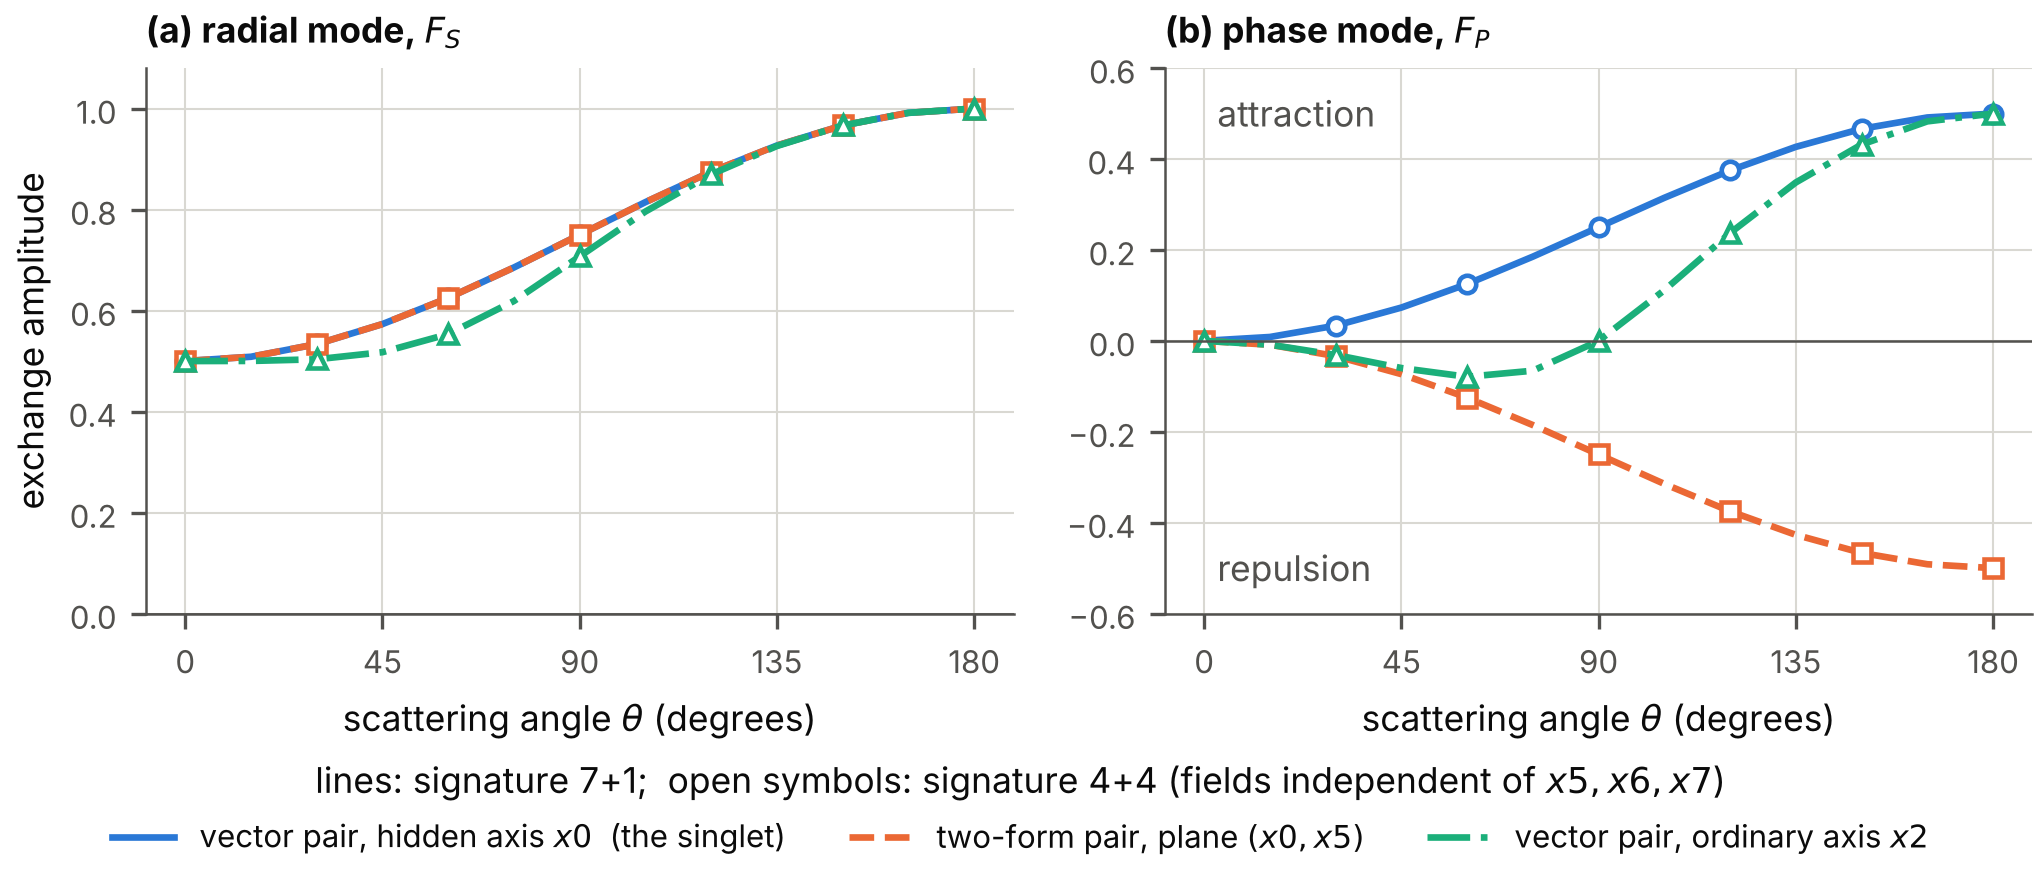
\includegraphics[width=1\textwidth,height=\textheight]{../figures/fig_kernels.png}
\caption{Exchange amplitudes of the two modes of the Vorton-Scalar in
three pair channels, for momenta of magnitude \(m\) in the plane
\((x1,x2)\), as functions of the scattering angle. Lines: 7+1; open
symbols: 4+4. The radial mode attracts in all channels; the phase mode
attracts in the vector channel along the hidden axis, repels in the
two-form channel, and has both signs for a vector pair polarized in the
plane of the momenta. Data: \texttt{data/pair\_channel\_kernel.csv};
program: \texttt{spacetimes\ channels}; drawn by
\texttt{make\_figures.py\ kernels}.}
\end{figure}

\begin{longtable}[]{@{}
  >{\raggedright\arraybackslash}p{(\columnwidth - 12\tabcolsep) * \real{0.2881}}
  >{\raggedleft\arraybackslash}p{(\columnwidth - 12\tabcolsep) * \real{0.1186}}
  >{\raggedleft\arraybackslash}p{(\columnwidth - 12\tabcolsep) * \real{0.1186}}
  >{\raggedleft\arraybackslash}p{(\columnwidth - 12\tabcolsep) * \real{0.1186}}
  >{\raggedleft\arraybackslash}p{(\columnwidth - 12\tabcolsep) * \real{0.1186}}
  >{\raggedleft\arraybackslash}p{(\columnwidth - 12\tabcolsep) * \real{0.1186}}
  >{\raggedleft\arraybackslash}p{(\columnwidth - 12\tabcolsep) * \real{0.1186}}@{}}
\toprule\noalign{}
\begin{minipage}[b]{\linewidth}\raggedright
pair channel (7+1)
\end{minipage} & \begin{minipage}[b]{\linewidth}\raggedleft
\(F_S\), 60°
\end{minipage} & \begin{minipage}[b]{\linewidth}\raggedleft
\(F_S\), 120°
\end{minipage} & \begin{minipage}[b]{\linewidth}\raggedleft
\(F_S\), 180°
\end{minipage} & \begin{minipage}[b]{\linewidth}\raggedleft
\(F_P\), 60°
\end{minipage} & \begin{minipage}[b]{\linewidth}\raggedleft
\(F_P\), 120°
\end{minipage} & \begin{minipage}[b]{\linewidth}\raggedleft
\(F_P\), 180°
\end{minipage} \\
\midrule\noalign{}
\endhead
\bottomrule\noalign{}
\endlastfoot
vector, hidden axis \(x0\) & +0.6250 & +0.8750 & +1.0000 & +0.1250 &
+0.3750 & +0.5000 \\
vector, extra axis \(x5\) & +0.6250 & +0.8750 & +1.0000 & +0.1250 &
+0.3750 & +0.5000 \\
two-form, plane \((x0,x5)\) & +0.6250 & +0.8750 & +1.0000 & -0.1250 &
-0.3750 & -0.5000 \\
two-form, plane \((x5,x6)\) & +0.6250 & +0.8750 & +1.0000 & -0.1250 &
-0.3750 & -0.5000 \\
vector, ordinary axis \(x2\) & +0.5534 & +0.8696 & +1.0000 & -0.0791 &
+0.2372 & +0.5000 \\
\end{longtable}

Momenta of magnitude \(m\) in the plane \((x1,x2)\). The same quantities
for 4+4 (fields independent of \(x5,x6,x7\)) differ from those for 7+1
by at most \(3.0\times10^{-16}\) over all 585 entries of
\texttt{data/pair\_channel\_kernel.csv}.

The results, all verified by the program and identical for the two
spacetimes (the largest difference between the two is given in the last
line of the table):

\textbf{(i) Closed forms for the hidden-axis vector pair}
(\(X=C^{-}\gamma^0\)). With \(E=\sqrt{m^2+p^2}\),
\(E'=\sqrt{m^2+p'^2}\):
\[\begin{aligned}F_S&=\frac{m^2(E+E')^2+E^2p'^2+E'^2p^2-2EE'\,\vec p\cdot\vec p\,'}{4E^2E'^2},\\
F_P&=\frac{(m^2-EE')^2+2(m^2-EE')\,\vec p\cdot\vec p\,'+m^2q^2+p^2p'^2}{4E^2E'^2}.\end{aligned}\tag{4.3}\]
For equal energies these reduce to
\[\boxed{\;F_S=\frac{4m^2+q^2}{4E^2},\qquad F_P=\frac{q^2}{4E^2}\qquad(X=C_{1671}^{-}\gamma_{1671}^0\ \text{and}\ X=C_{1644}^{-}\gamma_{1644}^0)\;}\tag{4.4}\]
(unit test \texttt{kernel::tests::hidden\_axis\_closed\_forms} compares
(4.3) with the matrices for 200 random momenta, on and off the energy
shell; the command \texttt{channels} checks (4.4) at every tabulated
point to \(10^{-9}\)).

\textbf{(ii) The radial mode does not distinguish the pair channels} in
which the pair has no component along the momenta: \(F_S\) is the same
for the vector pairs along the four extra axes and for the two-form
pairs.

\textbf{(iii) The phase mode does.} For the vector pairs along the four
extra axes the amplitude is \(F_P=+q^2/4E^2\) (equal energies):
attraction at all angles. For the two-form pairs of the extra axes it is
\(F_P=-q^2/4E^2\): \textbf{repulsion} at all angles. For a vector pair
polarized along an axis of ordinary space the amplitude depends on the
directions of the momenta relative to that axis and takes both signs
(the third curve of Fig. 1); such a pair has ordinary spin 1 and is not
a candidate for the state sought here.

\textbf{(iv) A contact attraction of Fermi type.} The phase mode is
massless, so its contribution to the pairing interaction of the
hidden-axis pair is \(-g_{VS}^2F_P/q^2=-g_{VS}^2/4E^2\), independent of
the momentum transfer:
\[\boxed{\;V_{\rm NC}=-\frac{g_{VS}^2}{4E^2}=-\frac{1}{4v_{VS}^2}\,\frac{m^2}{E^2}=-\frac{G_{VS}}{2\sqrt2}\,\frac{m^2}{E^2}\;}\tag{4.5}\]
The neutral current (1.7) thus produces, between two fermions in the
hidden-axis singlet channel, a point-like attraction whose strength is
set by \(G_{VS}\) alone --- the direct analogue of Fermi's contact
interaction --- and an equally strong repulsion in the two-form
channels.

\textbf{(v) Low-energy limit.} For momenta small compared with \(m\),
\(F_S\to1\): the radial mode gives the attractive Yukawa potential
\[V_s(r)=-\alpha_{VS}\,\frac{e^{-m_sr}}{r},\qquad\alpha_{VS}=\frac{g_{VS}^2}{4\pi},\tag{4.6}\]
between any two fermions, whatever their internal states.

Together, (ii)--(iv) are the dynamical reason for the state proposed in
the task: the radial mode binds, and the neutral current selects, among
the 28 possible s-wave pairs (DM, Sec. 3.2), the four vector pairs along
the extra axes --- which are exactly the pairs of ordinary spin 0 that
form a 4-vector --- and penalizes the six spin-0 two-form pairs.

\emph{What Sec. 5 needs:} the amplitudes (4.3).

\begin{center}\rule{0.5\linewidth}{0.5pt}\end{center}

\hypertarget{the-gap-equation}{%
\section{5. The gap equation}\label{the-gap-equation}}

\hypertarget{derivation-from-the-effective-action-of-cornwall-jackiw-and-tomboulis}{%
\subsection{5.1 Derivation from the effective action of Cornwall, Jackiw
and
Tomboulis}\label{derivation-from-the-effective-action-of-cornwall-jackiw-and-tomboulis}}

At a fermion density \(n\), with a chemical potential \(\mu\) for the
conserved fermion number, the attraction of Sec. 4 makes the Fermi sea
unstable against the formation of pairs. The standard tool for such a
state is the effective action for composite operators of Cornwall,
Jackiw and Tomboulis (CJT), a functional \(\Gamma[S]\) of the full
fermion propagator \(S\) whose stationary point is the true propagator.
In the doubled (Nambu--Gor'kov) description,
\(\Psi=(\psi,\psi^{\dagger T})\), the propagator has off-diagonal blocks
that describe pair correlations, and
\[\Gamma[S]=-\frac i2\,\mathrm{Tr}\ln S^{-1}-\frac i2\,\mathrm{Tr}\big(S_0^{-1}S-1\big)+\Gamma_2[S],\tag{5.1}\]
where \(S_0\) is the free propagator, \(\Gamma_2\) is the sum of the
two-particle irreducible vacuum diagrams, and the factors \(\tfrac12\)
compensate the doubling of the field. (Supplement S4 derives the method,
states this action for the present models with all its variables, and
uses it for independent checks of the results of this section and for
further predictions.) We keep in \(\Gamma_2\) the diagram with one
exchanged boson (radial mode plus phase mode), and make three further
approximations, each of them standard and each stated here because the
results depend on them:

\begin{enumerate}
\def\labelenumi{\arabic{enumi}.}
\tightlist
\item
  \emph{static exchange}: the boson propagators are evaluated at zero
  energy transfer;
\item
  \emph{no change of the normal state}: the diagonal part of the
  self-energy is absorbed into \(m\) and \(\mu\);
\item
  \emph{particles only}: the pairing of antiparticle states is
  neglected, which is valid when the gap and the temperature are small
  compared with \(m\).
\end{enumerate}

The stationarity condition \(\delta\Gamma/\delta S=0\) then becomes a
linear relation between the off-diagonal self-energy (the gap) and the
pair correlation, and for a gap matrix proportional to the two-particle
content of one pair operator \(X\),
\(\Delta(\vec k)\,\Phi_X(\vec k)/\sqrt{N_X/8}\), it reduces to
\[\begin{aligned}\Delta(k)&=\frac{1}{4\pi^2}\int_0^\infty dk'\,k'^2\;W(k,k')\;\frac{\Delta(k')}{E_\Delta(k')}\,\tanh\frac{E_\Delta(k')}{2T},\\
E_\Delta(k)&=\sqrt{\xi_k^2+\Delta(k)^2},\qquad\xi_k=\sqrt{m^2+k^2}-\mu,\end{aligned}\tag{5.2}\]
\[W(k,k')=\frac12\int_{-1}^{1}d\cos\theta\;g_{VS}^2\left[\frac{F_S}{q^2+m_s^2}+\sigma_X\,\frac{F_P}{q^2}\right],\qquad q^2=k^2+k'^2-2kk'\cos\theta,\tag{5.3}\]
with \(F_S\), \(F_P\) of Eq. (4.3) and \(\sigma_X=+1\) for the vector
pairs along the extra axes, \(\sigma_X=-1\) for their two-form pairs.
For these channels the gap matrix is \emph{unitary} (Sec. 6): all eight
internal states have the same gap, which is why a single function
\(\Delta(k)\) suffices. The angular integral in (5.3) is done in closed
form (unit test
\texttt{gap::tests::angular\_average\_matches\_quadrature}). The
chemical potential is kept at its value without pairing,
\(\mu=\sqrt{m^2+k_F^2}\), where \(k_F\) is the Fermi momentum,
\(n=8\,k_F^3/6\pi^2\) for eight internal states; this is correct as long
as the gap is small compared with the Fermi kinetic energy
\(E_F=\sqrt{m^2+k_F^2}-m\) (the \emph{weak-coupling} or BCS regime).

\hypertarget{numerical-solution-and-its-validation}{%
\subsection{5.2 Numerical solution, and its
validation}\label{numerical-solution-and-its-validation}}

\texttt{spacetimes\ gap} solves (5.2) by iteration on a momentum grid
that is refined logarithmically around \(k_F\) (\texttt{gap.rs}), for
120 combinations of \(g_{VS}\), \(m_s/m\) and \(k_F/m\), for three
kernels: the vector channel (\(\sigma_X=+1\)), the radial mode alone,
and the two-form channel (\(\sigma_X=-1\)). The critical temperature
\(T_c\) is the temperature at which the linearized equation has the
eigenvalue 1. Two validations:

\begin{itemize}
\tightlist
\item
  for a kernel that is constant in a shell around the Fermi surface the
  program reproduces the textbook results
  \(\Delta=2\omega_c\,e^{-1/\lambda}\) and \(T_c=0.567\,\Delta\) (unit
  test \texttt{gap::tests::bcs\_shell\_model});
\item
  in the scan, the ratio \(T_c/\Delta(k_F)\) lies within 0.03 of 0.567
  wherever the coupling is weak (checked by the command; column
  \texttt{Tc\_over\_gap\_V} of \texttt{data/gap\_scan.csv}).
\end{itemize}

\begin{figure}
\centering
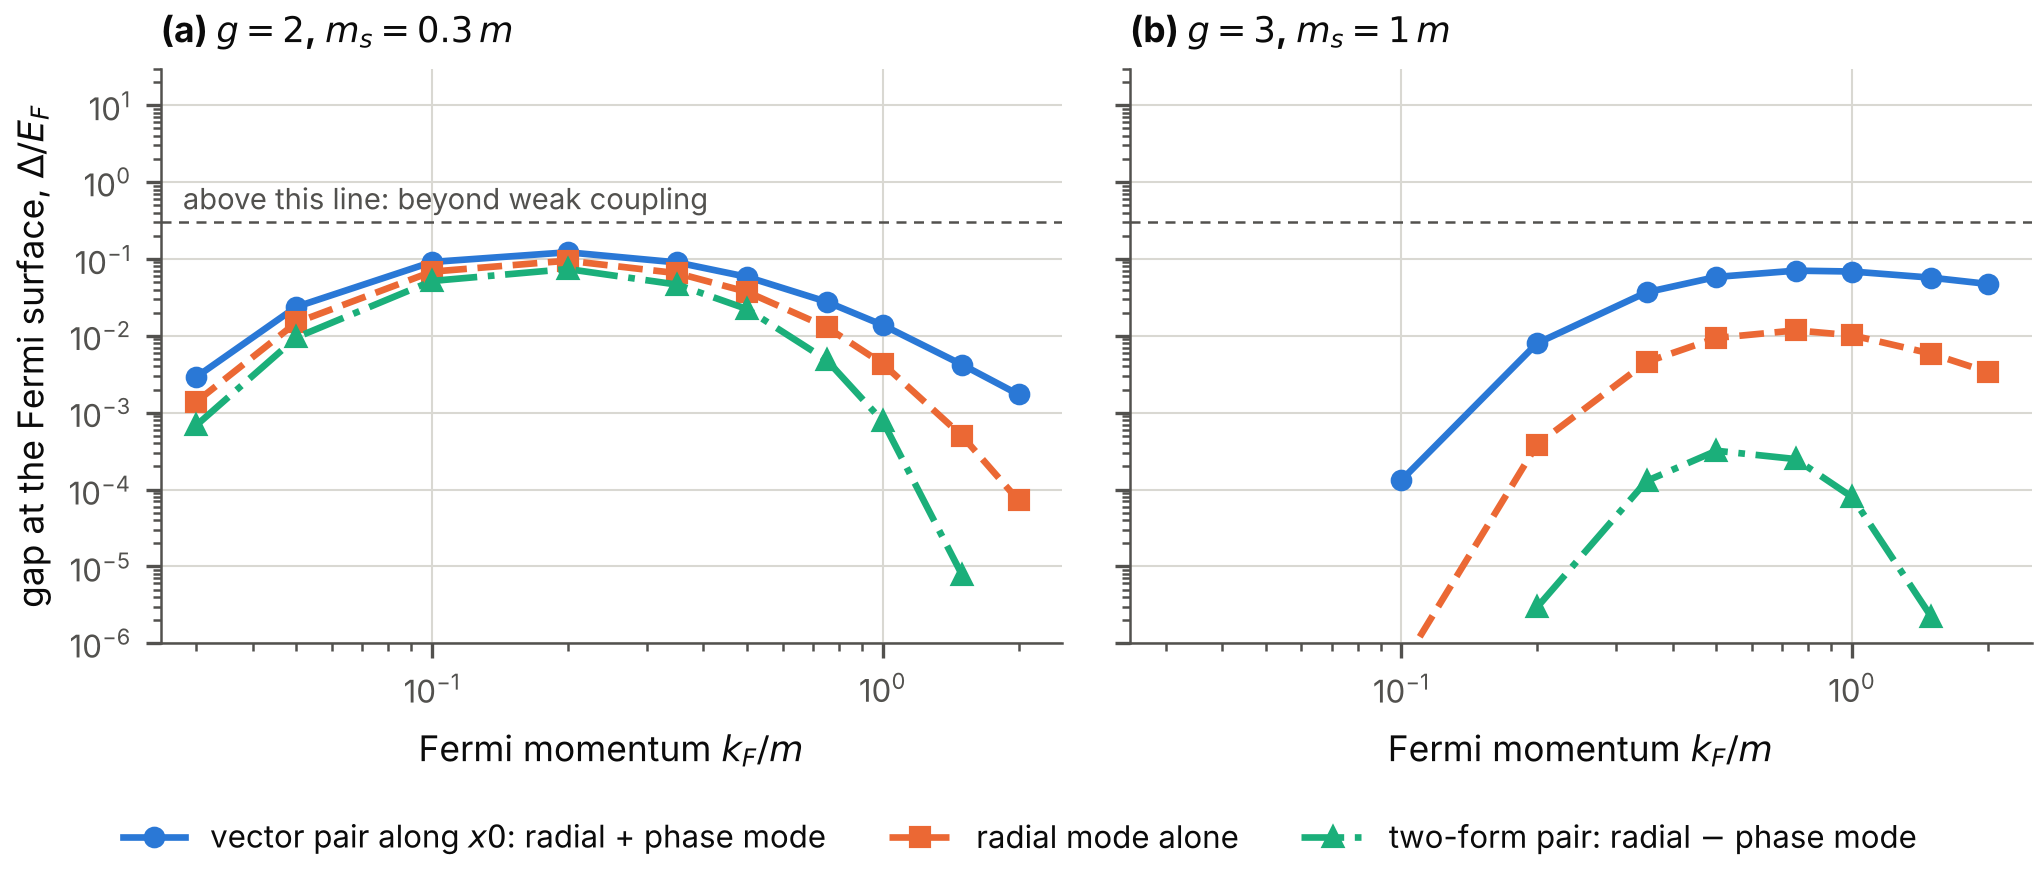
\includegraphics[width=1\textwidth,height=\textheight]{../figures/fig_gap.png}
\caption{Gap at the Fermi surface in units of the Fermi kinetic energy,
as a function of the Fermi momentum, for two sets of couplings. In every
case the vector pair along an extra axis, to which the radial mode and
the phase mode both contribute attraction, has the largest gap; the
two-form pair, in which the phase mode repels, has the smallest. Open
symbols mark points above the dashed line, where the gap is no longer
small compared with the Fermi energy and Eq. (5.2) with a fixed chemical
potential is not quantitative. Data: \texttt{data/gap\_scan.csv};
program: \texttt{spacetimes\ gap}.}
\end{figure}

\begin{longtable}[]{@{}
  >{\raggedleft\arraybackslash}p{(\columnwidth - 18\tabcolsep) * \real{0.0595}}
  >{\raggedleft\arraybackslash}p{(\columnwidth - 18\tabcolsep) * \real{0.0714}}
  >{\raggedleft\arraybackslash}p{(\columnwidth - 18\tabcolsep) * \real{0.0714}}
  >{\raggedleft\arraybackslash}p{(\columnwidth - 18\tabcolsep) * \real{0.0833}}
  >{\raggedleft\arraybackslash}p{(\columnwidth - 18\tabcolsep) * \real{0.0952}}
  >{\raggedleft\arraybackslash}p{(\columnwidth - 18\tabcolsep) * \real{0.1310}}
  >{\raggedleft\arraybackslash}p{(\columnwidth - 18\tabcolsep) * \real{0.1310}}
  >{\raggedleft\arraybackslash}p{(\columnwidth - 18\tabcolsep) * \real{0.1310}}
  >{\raggedleft\arraybackslash}p{(\columnwidth - 18\tabcolsep) * \real{0.1071}}
  >{\raggedright\arraybackslash}p{(\columnwidth - 18\tabcolsep) * \real{0.1190}}@{}}
\toprule\noalign{}
\begin{minipage}[b]{\linewidth}\raggedleft
\(g_{VS}\)
\end{minipage} & \begin{minipage}[b]{\linewidth}\raggedleft
\(m_s/m\)
\end{minipage} & \begin{minipage}[b]{\linewidth}\raggedleft
\(k_F/m\)
\end{minipage} & \begin{minipage}[b]{\linewidth}\raggedleft
\(\lambda_S\)
\end{minipage} & \begin{minipage}[b]{\linewidth}\raggedleft
\(\lambda_P\)
\end{minipage} & \begin{minipage}[b]{\linewidth}\raggedleft
vector: \(\Delta/E_F\)
\end{minipage} & \begin{minipage}[b]{\linewidth}\raggedleft
radial only
\end{minipage} & \begin{minipage}[b]{\linewidth}\raggedleft
two-form
\end{minipage} & \begin{minipage}[b]{\linewidth}\raggedleft
\(T_c/\Delta\) (vector)
\end{minipage} & \begin{minipage}[b]{\linewidth}\raggedright
coupling
\end{minipage} \\
\midrule\noalign{}
\endhead
\bottomrule\noalign{}
\endlastfoot
1 & 0.1 & 0.1 & 0.204 & 0.0013 & \(2.5\times10^{-2}\) &
\(2.4\times10^{-2}\) & \(2.3\times10^{-2}\) & 0.567 & weak \\
1 & 0.1 & 0.35 & 0.137 & 0.0042 & \(1.4\times10^{-3}\) &
\(1.1\times10^{-3}\) & \(8.4\times10^{-4}\) & 0.567 & weak \\
1 & 0.1 & 1 & 0.063 & 0.0090 & \(8.2\times10^{-7}\) & \(<10^{-7}\) &
\(<10^{-7}\) & 0.567 & weak \\
2 & 0.3 & 0.1 & 0.186 & 0.0050 & \(9.1\times10^{-2}\) &
\(6.8\times10^{-2}\) & \(5.2\times10^{-2}\) & 0.565 & weak \\
2 & 0.3 & 0.35 & 0.266 & 0.0167 & \(9.0\times10^{-2}\) &
\(6.5\times10^{-2}\) & \(4.6\times10^{-2}\) & 0.565 & weak \\
2 & 0.3 & 1 & 0.169 & 0.0358 & \(1.4\times10^{-2}\) &
\(4.3\times10^{-3}\) & \(7.7\times10^{-4}\) & 0.567 & weak \\
3 & 1 & 0.1 & 0.045 & 0.0113 & \(1.3\times10^{-4}\) &
\(4.9\times10^{-7}\) & \(<10^{-7}\) & 0.567 & weak \\
3 & 1 & 0.35 & 0.130 & 0.0377 & \(3.7\times10^{-2}\) &
\(4.6\times10^{-3}\) & \(1.3\times10^{-4}\) & 0.567 & weak \\
3 & 1 & 1 & 0.178 & 0.0806 & \(6.9\times10^{-2}\) & \(1.0\times10^{-2}\)
& \(8.0\times10^{-5}\) & 0.566 & weak \\
\end{longtable}

\(\lambda_S\) and \(\lambda_P\) are the dimensionless couplings
\(N(0)W(k_F,k_F)\) of the radial and of the phase mode. ``\(<10^{-7}\)''
means below the resolution of the calculation. Source:
\texttt{data/gap\_scan.csv} (all 120 combinations).

The table and Fig. 2 show the result that matters for the task:
\textbf{the gap of the vector channel exceeds that of the two-form
channel}, by a factor that grows with the density and with the mass of
the radial mode --- from a factor of a few to several orders of
magnitude. The phase mode alone (the neutral current without the radial
mode) gives a gap that is negligible at low density, because its
dimensionless coupling \(\lambda_P=N(0)\,g_{VS}^2/4E_F'^2\) (with
\(N(0)=k_FE_F'/2\pi^2\) the density of states per internal state and
\(E_F'=\sqrt{m^2+k_F^2}\)) vanishes with \(k_F\); it becomes comparable
to the radial contribution when \(k_F\sim m\).

\hypertarget{from-overlapping-pairs-to-bound-pairs}{%
\subsection{5.3 From overlapping pairs to bound
pairs}\label{from-overlapping-pairs-to-bound-pairs}}

At low density the attraction (4.6) is felt by two fermions alone. They
form a bound state if and only if (\texttt{spacetimes\ dimer};
\texttt{data/dimer.csv}; Fig. 3)
\[\boxed{\;D_{VS}\equiv\frac{\alpha_{VS}\,m}{m_s}>D_c=\,1.67981\;}\tag{5.4}\]
The program integrates the radial Schrödinger equation
\(u''+D_{VS}\,e^{-\rho}u/\rho=\varepsilon u\) (\(\rho=m_sr\),
\(\varepsilon=mE_b/m_s^2\), \(E_b\) the binding energy); the critical
value agrees with the value 1.6798 known for the Yukawa potential, the
scattering length has the Born limit \(a=-D_{VS}/m_s\) for weak
coupling, and the binding energy approaches the screened-Coulomb
expansion \(\varepsilon=D_{VS}^2/4-D_{VS}+3/2-2/D_{VS}\) for strong
coupling (unit tests of \texttt{dimer.rs}).

\begin{figure}
\centering
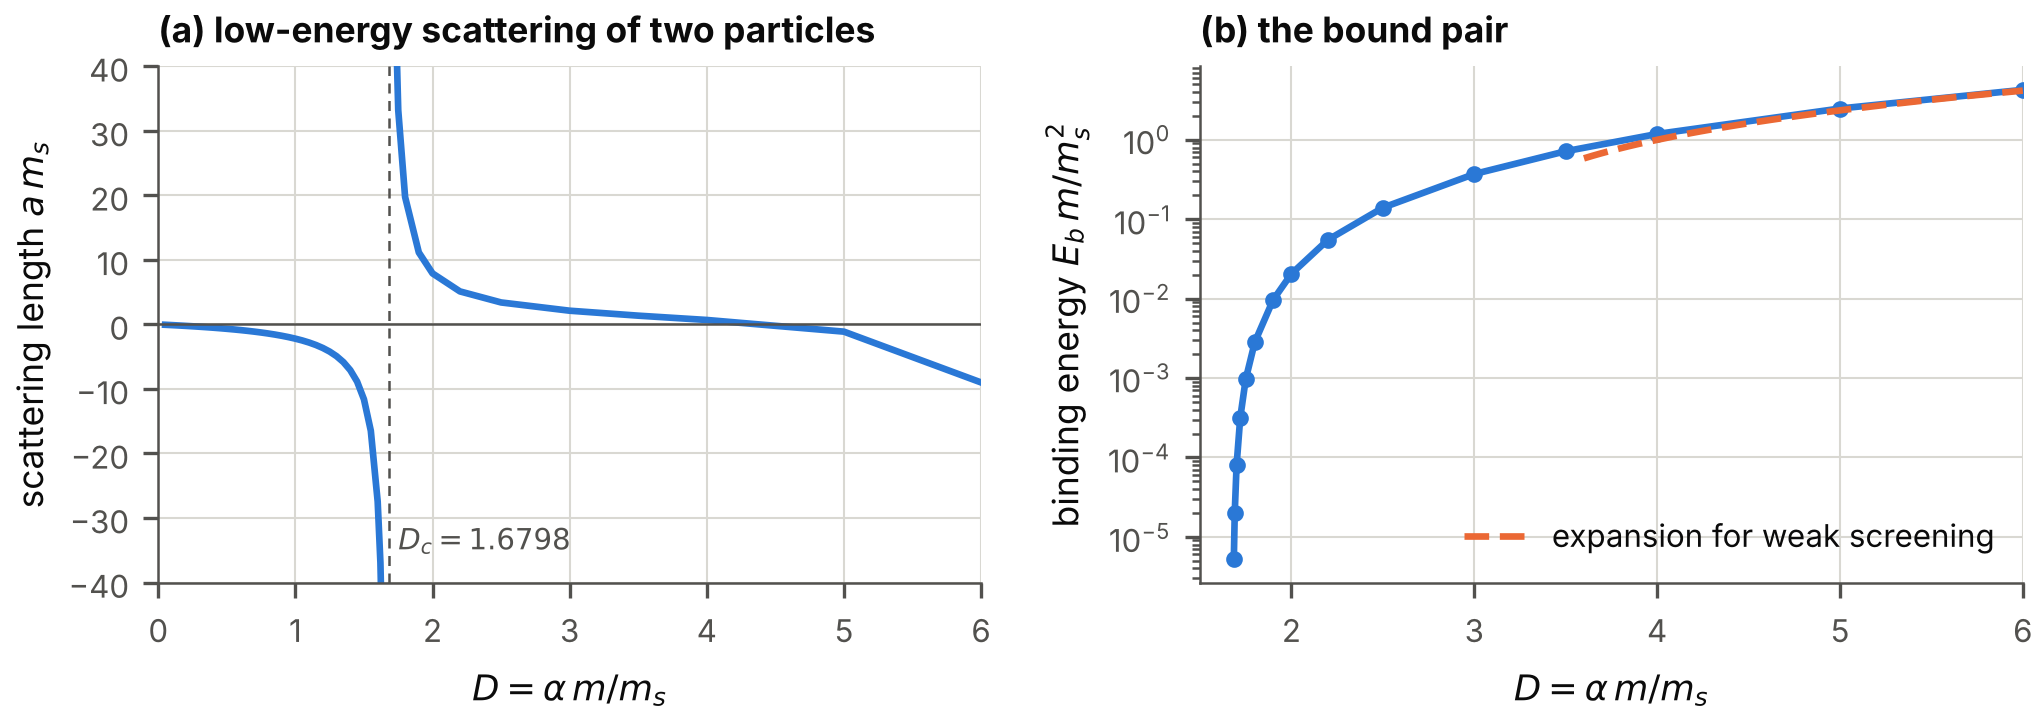
\includegraphics[width=1\textwidth,height=\textheight]{../figures/fig_dimer.png}
\caption{(a) Scattering length of two fermions in the Yukawa potential
of the radial mode, in units of \(1/m_s\); it diverges at the critical
coupling, where the bound state appears. (b) Binding energy of the pair.
Data: \texttt{data/dimer.csv}; program: \texttt{spacetimes\ dimer}.}
\end{figure}

For \(D_{VS}<D_c\) the superfluid is of the BCS kind at all densities:
large, overlapping pairs, described by Eq. (5.2). For \(D_{VS}>D_c\) a
dilute gas consists of bound pairs --- bosons of spin 0 --- that
condense; as the density rises the pairs overlap and the state crosses
over continuously to the BCS kind. In the scan of Sec. 5.2 the points
marked ``beyond weak coupling'' are on the way to this regime; there the
\emph{existence} of the paired state is not in doubt (two fermions
already bind), but the numbers of Eq. (5.2) are not quantitative. With
eight internal states and an attraction between all of them, bound
states of more than two fermions are to be expected as well; they are
discussed in Supplement S3, Sec. 4.

\emph{What Sec. 6 needs:} the statement that the four vector pairs along
the extra axes have the strongest pairing.

\begin{center}\rule{0.5\linewidth}{0.5pt}\end{center}

\hypertarget{the-order-parameter-and-the-ground-state}{%
\section{6. The order parameter and the ground
state}\label{the-order-parameter-and-the-ground-state}}

\hypertarget{the-gap-matrix}{%
\subsection{6.1 The gap matrix}\label{the-gap-matrix}}

The condensate is described by the expectation values of the four vector
pair operators along the extra axes,
\[\Delta^a\propto\big\langle\psi^TC^{-}\gamma^a\psi\big\rangle,\qquad a\in\{0,5,6,7\},\]
four complex numbers. On the eight internal states of the pair
\((\vec p,-\vec p)\) they define the \textbf{gap matrix}
\[\mathsf M(\vec p)=\sum_{a}\Delta^a\,\frac{\Phi_a(\vec p)}{\sqrt{N_a/8}},\qquad\Phi_a=U(\vec p)^TC^{-}\gamma^aU(-\vec p),\tag{6.1}\]
and the energies of the quasi-particles are \(\sqrt{\xi^2+d_r^2}\),
where \(d_r^2\) (\(r=1,\dots,8\)) are the eigenvalues of
\(\mathsf M\mathsf M^\dagger\).

\hypertarget{the-ginzburglandau-energy}{%
\subsection{6.2 The Ginzburg--Landau
energy}\label{the-ginzburglandau-energy}}

Near the critical temperature the free energy can be expanded in the
order parameter (Ginzburg and Landau). At weak coupling the expansion is
\[\begin{aligned}\mathcal F&=a(T)\,\mathrm{Tr}\big[\mathsf M\mathsf M^\dagger\big]+\frac b2\,\mathrm{Tr}\big[(\mathsf M\mathsf M^\dagger)^2\big]+K\,\mathrm{Tr}\big[\nabla\mathsf M\cdot\nabla\mathsf M^\dagger\big]+\dots,\\
a(T)&=\frac{N(0)}2\ln\frac{T}{T_c},\qquad b=\frac{7\zeta(3)}{16\pi^2T_c^2}N(0)>0,\end{aligned}\]
with \(N(0)\) the density of states at the Fermi surface per internal
state (for a unitary state \(\mathsf M\mathsf M^\dagger=|\Delta|^2\)
this is the textbook energy of four independent copies of a
spin-\(\tfrac12\) superconductor, with the minimum
\(|\Delta|^2=\frac{8\pi^2}{7\zeta(3)}T_c^2(1-T/T_c)\)), so the form of
the quartic term is decided by one matrix identity. The program verifies
it for both spacetimes (\texttt{spacetimes\ channels}; unit test
\texttt{kernel::tests::ginzburg\_landau\_quartic\_invariant};
\texttt{data/gl\_quartic\_check.csv}; largest deviation
\(2.1\times10^{-14}\) for 7+1 and \(1.8\times10^{-14}\) for 4+4):
\[\boxed{\;\frac18\mathrm{Tr}\big[\mathsf M\mathsf M^\dagger\big]=\sum_a|\Delta^a|^2,\qquad
\frac18\mathrm{Tr}\big[(\mathsf M\mathsf M^\dagger)^2\big]=2\Big(\sum_a|\Delta^a|^2\Big)^2-\big|\eta_{ab}\,\Delta^a\Delta^b\big|^2\;}\tag{6.2}\]
where \(\eta_{ab}\) is the metric of the spacetime restricted to the
four extra axes: \(\eta_{1671}=\mathrm{diag}(-1,-1,-1,-1)\) on them (all
four are space-like), and \(\eta_{1644}=\mathrm{diag}(+1,-1,-1,-1)\)
(the hidden axis is space-like, the other three are time-like). The
signature of the spacetime thus enters the energy of the superfluid
through the quadratic form \(\eta_{ab}\Delta^a\Delta^b\).

\emph{Origin of (6.2) in 7+1.} For particles at rest
\(\Phi_a=-\tau_{1671}^a\) (check \texttt{71-Q9}), real antisymmetric 8×8
matrices that anticommute and square to \(-1\). Then
\(\mathsf M\mathsf M^\dagger=\sum_a|\Delta^a|^2-\sum_{a<b}(\Delta^a\Delta^{b*}-\Delta^b\Delta^{a*})\tau^a\tau^b\),
and since the products \(\tau^a\tau^b\) are traceless and mutually
trace-orthogonal with \((\tau^a\tau^b)^2=-1\), the trace of the square
is
\(8(\sum|\Delta^a|^2)^2+8\sum_{a<b}|\Delta^a\Delta^{b*}-\Delta^b\Delta^{a*}|^2\),
which equals \(8[2(\sum|\Delta|^2)^2-|\sum_a(\Delta^a)^2|^2]\).

\hypertarget{the-ground-state}{%
\subsection{6.3 The ground state}\label{the-ground-state}}

At fixed \(\sum_a|\Delta^a|^2\) the quartic term (6.2) is smallest when
\(|\eta_{ab}\Delta^a\Delta^b|\) is largest, i.e.~equal to
\(\sum_a|\Delta^a|^2\). Then
\(\mathsf M\mathsf M^\dagger=\sum_a|\Delta^a|^2\cdot1\): the state is
\textbf{unitary}, all eight quasi-particle branches have the same gap,
and the condensation energy is the largest possible. The minimizing
configurations are

\begin{itemize}
\tightlist
\item
  in 7+1: \(\Delta^a=|\Delta|\,e^{i\varphi}\,n^a\) with a \emph{real}
  unit vector \(n^a\) in the space of the four extra axes;
\item
  in 4+4: \(\Delta^0=|\Delta|e^{i\varphi}\,n^0\),
  \(\Delta^t=\pm i\,|\Delta|e^{i\varphi}\,n^t\) with a real unit vector
  \((n^0,n^5,n^6,n^7)\): the components along the time-like axes carry a
  relative phase \(\pm i\).
\end{itemize}

The \textbf{hidden-axis singlet} of the task,
\[\boxed{\;\begin{aligned}&\Delta^a=\Delta\,\delta^{a0}:\\
&\langle\psi_{1671}^TC_{1671}^{-}\gamma_{1671}^0\psi_{1671}\rangle\neq0\quad\text{(7+1)},\qquad\langle\psi_{1644}^TC_{1644}^{-}\gamma_{1644}^0\psi_{1644}\rangle\neq0\quad\text{(4+4)},\end{aligned}\;}\tag{6.3}\]
is a member of this family in both spacetimes. Its properties, proved in
``dirac matrices'' (Sec. 3.3): the pair has ordinary spin 0; it is
invariant under the rotations of ordinary space and of the coordinates
\(x5,x6,x7\); and it is invariant under the Lorentz transformations of
the seven coordinates other than \(x0\) --- in particular it is a
\emph{scalar} in ordinary spacetime, although it is a component of a
vector in eight dimensions.

\textbf{How the hidden axis is singled out.} By Sec. 2.1 the order
parameter is a 4-vector of the internal \(SO(4)\) of the zero-mode
sector in both spacetimes; in 4+4 the components that form the real
4-vector are \((\Delta^0,i\Delta^5,i\Delta^6,i\Delta^7)\), which is why
the relative phase \(\pm i\) appears above. All directions of this
4-vector have exactly the same energy.

\begin{itemize}
\tightlist
\item
  \emph{In 7+1} the direction \(n^a\) is chosen spontaneously, and
  calling the chosen one ``the hidden axis'' is a choice of coordinates.
  The symmetry breaking is \(SO(4)\to SO(3)\) together with
  \(U(1)_F\to Z_2\); besides the sound mode of the superfluid (the
  Goldstone mode of \(U(1)_F\)) there are three Goldstone modes, the
  rotations of \(n^a\). Because the \(SO(4)\) is a symmetry of the full
  theory, nothing within the 7+1 model prefers one direction.
\item
  \emph{In 4+4} the same holds within the zero-mode sector: the singlet
  \(\Delta^0\) of the rotations \(SO(3)_T\) of the additional times and
  their triplet \(\Delta^t\) are degenerate \textbf{exactly}, to all
  orders, because the hidden \(SO(4)\) of Sec. 2.1 rotates one into the
  other; the same four gapless modes exist. But the hidden symmetry is a
  property of the zero-mode sector only. Every effect that involves a
  dependence of the fields on \(x0\) --- in Stage 2, excitations that
  travel around the hidden ring, with energies of at least the inverse
  radius --- breaks it down to \(SO(3)_T\), under which the hidden axis
  \emph{is} distinguished. Such effects lift the degeneracy between
  singlet and triplet and give the three additional modes a mass. Which
  of the two then lies lower has not been determined; that it is the
  singlet (6.3) is the hypothesis of the task.
\end{itemize}

(An earlier version of this supplement called the degeneracy in 4+4
accidental. That was wrong; the symmetry analysis of Sec. 2.1, made in
the course of the checks of Supplement S4, corrected it. Error log,
E26.)

In Stage 2 of the author's programme the hidden coordinate is curled up
and the other three coordinates are treated differently; this breaks the
\(SO(4)\) of 7+1 explicitly as well, and would decide the direction in
both spacetimes. It is not implemented here.

\hypertarget{collective-modes-and-the-sound-of-the-superfluid}{%
\subsection{6.4 Collective modes and the sound of the
superfluid}\label{collective-modes-and-the-sound-of-the-superfluid}}

The phase \(\varphi\) of the order parameter is the Goldstone field of
the broken fermion number. Its excitation is a density wave, the first
sound of the superfluid (the Bogoliubov--Anderson mode), with the
velocity given by the compressibility, \(c_s^2=dP/d\rho\). In the
weak-coupling regime the pressure is the degeneracy pressure of the
fermions, and
\[c_s^2=\frac{k_F^2}{3\,(m^2+k_F^2)}=\frac{v_F^2}{3}\quad\text{(weak coupling)};\qquad c_s^2=\frac{4\pi a_{BB}\,n_B}{m_B^2}\quad\text{(dilute gas of bound pairs)},\tag{6.4}\]
where \(v_F\) is the Fermi velocity and, in the second expression
(Bogoliubov), \(m_B\), \(n_B\) and \(a_{BB}>0\) are the mass, the
density and the mutual scattering length of the bound pairs. Equation
(6.4) is the input of the cosmological simulations of Supplement S3, in
which the superfluid appears as a fluid with this sound speed.

\begin{center}\rule{0.5\linewidth}{0.5pt}\end{center}

\hypertarget{the-superfluid-field-equations-summary}{%
\section{7. The superfluid field equations
(summary)}\label{the-superfluid-field-equations-summary}}

For the reader who wants the complete set of equations in one place.
\emph{Normal phase, 7+1}: Eqs. (1.8); \emph{normal phase, 4+4 (quantized
sector)}: Eqs. (3.2). \emph{Paired phase}, both spacetimes, in the
mean-field approximation of Sec. 5: the fermion field obeys the
Bogoliubov--de Gennes equations
\[i\partial_4\psi=(\mathsf h-\mu)\,\psi+\hat\Delta\,\psi^{\dagger T},\qquad
\hat\Delta(\vec p)=U(\vec p)^{*}\,\mathsf M(\vec p)\,U(-\vec p)^{\dagger},\tag{7.1}\]
in which \(\hat\Delta\) is the 16×16 pair potential built from the gap
matrix (6.1), and the gap obeys the self-consistency equation (5.2) with
the kernel (5.3). Near \(T_c\) the order parameter varies slowly and
obeys the Ginzburg--Landau equation that follows from Sec. 6.2,
\[-K\,\nabla^2\Delta^a+a(T)\,\Delta^a+b\Big[2\Big(\sum_c|\Delta^c|^2\Big)\Delta^a-\big(\eta_{cd}\Delta^c\Delta^d\big)\,\eta_{ab}\,\Delta^{b*}\Big]=0,\qquad K=\frac{7\zeta(3)}{96\pi^2T_c^2}N(0)\,v_F^2,\tag{7.2}\]
obtained by varying the energy of Sec. 6.2 with respect to
\(\Delta^{a*}\) and using (6.2). For a uniform unitary state it gives
\(a+b|\Delta|^2=0\), the minimum quoted in Sec. 6.2. The stiffness \(K\)
is the standard weak-coupling value for an isotropic unitary state (it
corresponds to the coherence length
\(\xi^2=K/|a|=7\zeta(3)v_F^2/[48\pi^2T_c^2(1-T/T_c)]\)); it has not been
re-derived for this model and is quoted for orientation only.

\begin{center}\rule{0.5\linewidth}{0.5pt}\end{center}

\hypertarget{vortices-and-vortons-what-the-name-refers-to}{%
\section{8. Vortices and vortons (what the name refers
to)}\label{vortices-and-vortons-what-the-name-refers-to}}

This section collects known results that apply to the Vorton-Scalar;
none of them is computed in this project, and each is attributed. Two
kinds of vortex must be kept apart.

\emph{Vortices of the superfluid.} The order parameter \(\Delta^a\) has
a phase, the Goldstone field of fermion number. A line around which this
phase winds by \(2\pi\) is a quantized vortex of the superfluid, with
circulation \(2\pi/(2m)\) per unit winding (Onsager, Feynman; the pair
has mass \(2m\)). In its core the condensate vanishes and the scalar
density of the fermions differs from its value in the bulk; by the
second of Eqs. (1.8) so does the Vorton-Scalar. Every such vortex
therefore carries a tube of displaced Vorton-Scalar field along with it.
This is the sense in which the scalar was named in the NCSS project.

\emph{Vortices of the Vorton-Scalar itself.} A complex scalar with the
potential of (1.1) has static solutions in which the phase winds by
\(2\pi n\) around a line and \(|\Phi_{VS}|\) vanishes on the line
(Nielsen and Olesen for the gauged case; for a global symmetry such as
\(U(1)_{VS}\) the energy per length grows logarithmically with the
distance).

\emph{Zero modes.} A fermion that obtains its mass from the scalar
through a Yukawa coupling of the form (1.1) is massless on the line, and
the Dirac equation in the background of the vortex has \(|n|\)
normalizable solutions of zero energy that move along the line at the
speed of light (Jackiw and Rossi). The first of Eqs. (1.8) is of exactly
this type.

\emph{Currents and vortons.} Zero modes make the string a perfect
conductor of the corresponding charge (Witten's superconducting strings;
here the charge is fermion number). A closed loop carrying such a
current has a conserved number of charge carriers and a conserved
winding of the current; the resulting angular momentum can balance the
tension of the string and prevent the loop from collapsing. Such
stationary loops are \textbf{vortons} (Davis and Shellard). Whether they
are stable, and with what abundance they would be produced, depends on
details that have been studied for other models and are open here. The
NCSS project used a real scalar, which has no such defects, and its
documents state that its Vorton-Scalar is unrelated to these vortons;
for the complex field of the present project the relation is literal,
but nothing below depends on it.

\emph{The hidden ring.} The author's hypothesis for Stage 2 is that
\(x0\) curls up into a ring. A Vorton-Scalar whose phase winds
\emph{around that ring}, \(\Phi_{VS}\propto e^{i\,n\,x0/R}\), is a
configuration with a constant neutral current \(J_{VS}^0=n\,v_{VS}^2/R\)
along the hidden axis. By (1.7) it acts on the fermions as a constant
axial potential along \(x0\). This is a natural object to study in Stage
2; nothing about it is claimed here.

\begin{center}\rule{0.5\linewidth}{0.5pt}\end{center}

\hypertarget{what-has-been-established-and-what-has-not}{%
\section{9. What has been established, and what has
not}\label{what-has-been-established-and-what-has-not}}

\textbf{Established} (each item with its evidence):

\begin{enumerate}
\def\labelenumi{\arabic{enumi}.}
\tightlist
\item
  A field with the required properties exists and is defined by the
  Lagrangian (1.1) in 7+1: a complex scalar whose neutral current (1.6)
  couples to the axial current of the fermions with a Fermi-type
  constant (1.7), and from which the fermion mass originates (1.5).
  (Algebra of Sec. 1; the matrix properties used are machine-checked.)
\item
  In 4+4 the same construction is impossible in the fully covariant
  theory (Sec. 3.1) and possible in the quantized sector of fields
  independent of the additional times (Sec. 3.2).
\item
  One-boson exchange is attractive in the hidden-axis vector channel for
  both modes, with the closed forms (4.4); the neutral current gives a
  contact attraction (4.5) in that channel and repulsion in the two-form
  channels. (Numerical evaluation from the matrices, both spacetimes;
  closed forms verified.)
\item
  The mean-field gap equation has solutions; the vector channel has the
  largest gap; the numerical method reproduces the textbook limits.
  (Sec. 5.)
\item
  Two fermions bind when \(D_{VS}>1.6798\). (Sec. 5.3.)
\item
  The quartic Ginzburg--Landau invariant is (6.2), with the metric of
  the spacetime; the hidden-axis singlet (6.3) is among the states of
  lowest energy. (Machine check, both spacetimes.)
\item
  In the sector of fields independent of the extra coordinates both
  models have the internal symmetry
  \(SU(2)_A\times SU(2)_B\times U(1)_F\times U(1)_E\), under which the
  order parameter is a 4-vector; in 4+4 this symmetry is hidden (Sec.
  2.1; machine check).
\end{enumerate}

\textbf{Not established:}

\begin{enumerate}
\def\labelenumi{\arabic{enumi}.}
\tightlist
\item
  That the hidden axis is \emph{preferred}: in 7+1 the direction is
  spontaneous; in 4+4 singlet and triplet are exactly degenerate in the
  zero-mode sector, and which is lower once the fields depend on \(x0\)
  has not been computed (Sec. 6.3).
\item
  Anything beyond the mean-field, static, particles-only approximation:
  retardation, the renormalization of the normal state, fluctuations of
  the order parameter, and the strong-coupling regime beyond the open
  symbols of Fig. 2.
\item
  The consistency of the 4+4 model with the full spacetime (the
  restriction to fields independent of \(x5,x6,x7\) is an assumption).
\item
  The high-energy completion of the theory (the couplings have negative
  mass dimension in eight dimensions).
\item
  Stability and abundance of vortons; anything about Stage 2.
\item
  Whether nature contains this field. The consequences for the Higgs
  hypothesis are examined in Supplement S2, those for cosmology in
  Supplement S3; Supplement S4 re-derives the results of Secs. 5 and 6
  from the effective action of Cornwall, Jackiw and Tomboulis and adds
  what that action predicts for the unpaired state, for finite
  temperature and for the vacuum.
\end{enumerate}

\begin{center}\rule{0.5\linewidth}{0.5pt}\end{center}

\hypertarget{provenance-of-the-numbers-and-figures}{%
\section{10. Provenance of the numbers and
figures}\label{provenance-of-the-numbers-and-figures}}

\begin{longtable}[]{@{}
  >{\raggedright\arraybackslash}p{(\columnwidth - 4\tabcolsep) * \real{0.2963}}
  >{\raggedright\arraybackslash}p{(\columnwidth - 4\tabcolsep) * \real{0.3704}}
  >{\raggedright\arraybackslash}p{(\columnwidth - 4\tabcolsep) * \real{0.3333}}@{}}
\toprule\noalign{}
\begin{minipage}[b]{\linewidth}\raggedright
Item
\end{minipage} & \begin{minipage}[b]{\linewidth}\raggedright
Produced by
\end{minipage} & \begin{minipage}[b]{\linewidth}\raggedright
File
\end{minipage} \\
\midrule\noalign{}
\endhead
\bottomrule\noalign{}
\endlastfoot
amplitudes \(F_S\), \(F_P\) (Fig. 1, table of Sec. 4.2) &
\texttt{spacetimes\ channels} &
\texttt{data/pair\_channel\_kernel.csv} \\
closed forms (4.3), (4.4) & unit test
\texttt{kernel::tests::hidden\_axis\_closed\_forms};
\texttt{spacetimes\ channels} & --- \\
gaps and critical temperatures (Fig. 2, table of Sec. 5.2) &
\texttt{spacetimes\ gap} & \texttt{data/gap\_scan.csv},
\texttt{data/gap\_profile.csv} \\
critical coupling, scattering length, binding energy (Fig. 3) &
\texttt{spacetimes\ dimer} & \texttt{data/dimer.csv} \\
identity (6.2) & \texttt{spacetimes\ channels}; unit test
\texttt{kernel::tests::ginzburg\_landau\_quartic\_invariant} &
\texttt{data/gl\_quartic\_check.csv} \\
internal symmetry (Sec. 2.1) & \texttt{spacetimes\ symmetry}; unit tests
of \texttt{symmetry.rs} & \texttt{data/reduced\_symmetry.csv} \\
figures &
\texttt{python3\ code/scripts/make\_figures.py\ kernels\ gap\ dimer} &
\texttt{figures/fig\_kernels}, \texttt{fig\_gap}, \texttt{fig\_dimer}
(.pdf, .png) \\
tables of this document & \texttt{python3\ code/scripts/make\_tables.py}
& \texttt{provenance/generated/tables.md} \\
\end{longtable}

\hypertarget{references}{%
\section{References}\label{references}}

\begin{enumerate}
\def\labelenumi{\arabic{enumi}.}
\tightlist
\item
  J. Bardeen, L. N. Cooper and J. R. Schrieffer, \emph{Theory of
  superconductivity}, Phys. Rev.~\textbf{108}, 1175 (1957).
\item
  Y. Nambu and G. Jona-Lasinio, \emph{Dynamical model of elementary
  particles based on an analogy with superconductivity. I}, Phys.
  Rev.~\textbf{122}, 345 (1961).
\item
  J. M. Cornwall, R. Jackiw and E. Tomboulis, \emph{Effective action for
  composite operators}, Phys. Rev.~D \textbf{10}, 2428 (1974).
\item
  J. Goldstone, \emph{Field theories with «superconductor» solutions},
  Nuovo Cimento \textbf{19}, 154 (1961).
\item
  M. L. Goldberger and S. B. Treiman, \emph{Decay of the pi meson},
  Phys. Rev.~\textbf{110}, 1178 (1958).
\item
  H. B. Nielsen and P. Olesen, \emph{Vortex-line models for dual
  strings}, Nucl. Phys. B \textbf{61}, 45 (1973).
\item
  R. Jackiw and P. Rossi, \emph{Zero modes of the vortex-fermion
  system}, Nucl. Phys. B \textbf{190}, 681 (1981).
\item
  E. Witten, \emph{Superconducting strings}, Nucl. Phys. B \textbf{249},
  557 (1985).
\item
  R. L. Davis and E. P. S. Shellard, \emph{Cosmic vortons}, Nucl. Phys.
  B \textbf{323}, 209 (1989).
\item
  N. N. Bogoliubov, \emph{On the theory of superfluidity}, J. Phys.
  (USSR) \textbf{11}, 23 (1947).
\item
  P. W. Anderson, \emph{Random-phase approximation in the theory of
  superconductivity}, Phys. Rev.~\textbf{112}, 1900 (1958).
\item
  A. J. Leggett, \emph{A theoretical description of the new phases of
  liquid \(^3\)He}, Rev.~Mod. Phys. \textbf{47}, 331 (1975) (unitary
  states and the weak-coupling Ginzburg--Landau energy of
  multi-component pair condensates).
\item
  L. Onsager, \emph{Statistical hydrodynamics}, Nuovo Cimento Suppl.
  \textbf{6}, 279 (1949); R. P. Feynman, \emph{Application of quantum
  mechanics to liquid helium}, Prog. Low Temp. Phys. \textbf{1}, 17
  (1955) (quantized vortices).
\item
  P. L. Nash, notebooks \texttt{4+4.nb} and \texttt{7+1.nb} (see
  \texttt{provenance/P3\_notebooks\_used}).
\end{enumerate}

\end{document}
